\documentclass{beamer}

\usepackage[utf8x]{inputenc}
\usepackage[T1]{fontenc}
\usepackage{graphicx}
\usepackage{amsthm,amssymb,amsbsy,amsmath,amsfonts,amssymb,amscd}
\usepackage{dsfont}
\usepackage{array}
\useoutertheme[subsection=false]{miniframes}
\usepackage{lmodern}

%%%%%%%%%%%%%%%%%%%%%%%%
% GENERAL BEAMER STYLE :

\setbeamertemplate{footline}{
  \hbox{%
    \begin{beamercolorbox}[wd=.2\paperwidth,ht=2ex,dp=1ex,left]{author in head/foot}%
      \hskip1em\usebeamerfont{author in head/foot}\insertshortauthor
    \end{beamercolorbox}%
    \begin{beamercolorbox}[wd=.6\paperwidth,ht=2ex,dp=1ex,center]{title in head/foot}%
      \usebeamerfont{title in head/foot}\insertshorttitle
    \end{beamercolorbox}%
    \begin{beamercolorbox}[wd=.2\paperwidth,ht=2ex,dp=1ex,right]{page number in head/foot}%
      \usebeamerfont{page number in head/foot}\insertframenumber{} / \inserttotalframenumber
      \kern1em 
    \end{beamercolorbox}
  }
}

\setbeamercolor{alerted text}{fg=red!80!black}
\setbeamercolor{itemize/enumerate subbody}{fg=gray!70!black}
\setbeamertemplate{itemize item}[square]
\setbeamertemplate{itemize subitem}[triangle]%{{\textendash}}
\setbeamerfont{itemize/enumerate subbody}{size=\footnotesize}
\setbeamerfont{itemize/enumerate subitem}{size=\footnotesize}

\setbeamertemplate{navigation symbols}{}

% \AtBeginSection{
% \begin{frame}
%     \begin{centering}
%     \begin{beamercolorbox}[sep=12pt,center]{part title}
%     \usebeamerfont{section title}\insertsection\par
%     \end{beamercolorbox}
%     \end{centering}
% \end{frame}
% }

\AtBeginSection[]
{
  \begin{frame}
   \tableofcontents[currentsection]
  \end{frame}
}

\setbeamercolor{author in head/foot}{fg=gray,bg=white}
\setbeamercolor{title in head/foot}{fg=gray,bg=white}
\setbeamercolor{page number in head/foot}{fg=gray,bg=white}
\setbeamercolor{section in head/foot}{bg=black,fg=gray}
\setbeamercolor{subsection in head/foot}{bg=black,fg=gray}

 

\title[Short intro to Demand Forecasting]{A short introduction to Demand Forecasting}
\author[Mines Saint-\'Etienne]{Mines Saint-\'Etienne -- Master Génie industriel}
\institute[2016-2017]{\texorpdfstring{Nicolas Durrande (durrande@emse.fr)}{}}
\date{\null}

%%%%%%%%%%%%%%%%%%%%%%%%%%%%%%%%%%%%%%%%%%%%%%%%%%%%%%
%%%%%%%%%%%%%%%%%%%%%%%%%%%%%%%%%%%%%%%%%%%%%%%%%%%%%%
%%%%%%%%%%%%%%%%%%%%%%%%%%%%%%%%%%%%%%%%%%%%%%%%%%%%%%
\begin{document}

%%%%%%%%%%%%%%%%%%%%%%%%%%%%%%%%%%%%%%%%%%%%%%%%%%%%%%
\begin{frame}
  \titlepage
\end{frame}

%%%%%%%%%%%%%%%%%%%%%%%%%%%%%%%%%%%%%%%%%%%%%%%%%%%%%%
\begin{frame}{}
\structure{Objectives of the course:}
\begin{itemize}
	\item Being able to recognize common patterns in time series
	\item Explain and apply various forecasting methods
	\item Being able to asses the quality of a forecast
\end{itemize}
This course is inspired from www.slideshare.net/knksmart/forecasting-slides \\ \vspace{5mm}
\end{frame}

% %%%%%%%%%%%%%%%%%%%%%%%%%%%%%%%%%%%%%%%%%%%%%%%%%%%%%%
% \begin{frame}{}
% \structure{Outline}
% \begin{enumerate}
% 	\item What is forecasting and why
% 	\item Forecasting based on time series
% 	\item Measuring the forecast accuracy
% 	\item Conclusion
% \end{enumerate}
% \end{frame}

%%%%%%%%%%%%%%%%%%%%%%%%%%%%%%%%%%%%%%%%%%%%%%%%%%%%%%
%%%%%%%%%%%%%%%%%%%%%%%%%%%%%%%%%%%%%%%%%%%%%%%%%%%%%%
\section{Context}

%%%%%%%%%%%%%%%%%%%%%%%%%%%%%%%%%%%%%%%%%%%%%%%%%%%%%%
\begin{frame}{}
\begin{block}{What is forecasting ?}
Forecasting is the process of making predictions for an event that has not been observed. A typical example is to estimate the value of a variable at a future date.
\end{block}

\begin{block}{Why do we need forecasting ?}
Most managerial decisions will be applied in a near or distant future. In many cases, it is thus important to have an idea of the future environment in which these decisions will be applied.
\end{block}

\begin{block}{Is forecasting difficult ?}
it really depends on the problem!
\end{block}

\end{frame}

%%%%%%%%%%%%%%%%%%%%%%%%%%%%%%%%%%%%%%%%%%%%%%%%%%%%%%
\begin{frame}{}
\begin{example}
\textbf{Forecasting in operation management:}
\begin{itemize}
	\item Predicting demands of new or existing products
	\item Predicting cost of materials
	\item ...
\end{itemize}
\vspace{5mm}
\textbf{Decisions requiring forecasting:}
\begin{itemize}
		\item Choosing new facility location
		\item Identifying labour requirement
		\item Projecting material requirement
		\item Creating maintenance schedules
\end{itemize}
\end{example}
\end{frame}

%%%%%%%%%%%%%%%%%%%%%%%%%%%%%%%%%%%%%%%%%%%%%%%%%%%%%%
\begin{frame}{}
Succesfull forecasting is a combination of science and art:
\begin{itemize}
	\item Science since it relies on rigorous mathematical methods
	\item Art because the decision maker uses his experience, logic and intuition to supplement the forecasting quantitative analysis.
\end{itemize}
\end{frame}

%%%%%%%%%%%%%%%%%%%%%%%%%%%%%%%%%%%%%%%%%%%%%%%%%%%%%%
\begin{frame}{}
There are two kinds of forecast types:\\
\vspace{5mm} 
\textbf{qualitative} where the forecast is based on opinions. We can cite expert opinion, sale force survey, consumer survey, Delphi method, ...\\
\vspace{5mm} 
\textbf{quantitative methods} where the forecast is based on data. Common examples are time series analysis and associative methods.\\
\vspace{10mm}

\begin{center}
\structure{The process of decision making usually uses both.}
\end{center}
\begin{block}{}
Forecast cannot predict the actual future value but it tries to \textbf{minimize the prediction error}.
\end{block}
\end{frame}

%%%%%%%%%%%%%%%%%%%%%%%%%%%%%%%%%%%%%%%%%%%%%%%%%%%%%%
\begin{frame}{}
Given the quantity to forecast and the time horizon, the main forecasting steps are :
\begin{itemize}
	\item Selecting the forecasting model(s)
	\item Validate the model
	\item Making the forecast
\end{itemize}
\vspace{5mm}
The choice of the forecasting model depends on the characteristics of the time series.
%We will now make a detailed overview of the quantitative forecasting methods.

\end{frame}

%%%%%%%%%%%%%%%%%%%%%%%%%%%%%%%%%%%%%%%%%%%%%%%%%%%%%%
\begin{frame}{}
A time series corresponds to the observations of a variable over a set of regularly spaced points.\\
% \vspace{1cm}
\begin{example}
 2 representations of the same time series
\begin{center}
  \begin{tabular}{|c|ccccccccc|}
  \hline
  t 	& 0		&  1 	&  2 	&   3 	&  4 	& 5 	& 6 	& ... 	& 19   \\ \hline
  y		&-2.19	&  -4.7	&  -1.1 &   4.2 &   1.8 &   4.8 &   5.7 & ... 	& 10.7 \\ \hline
  \end{tabular}
  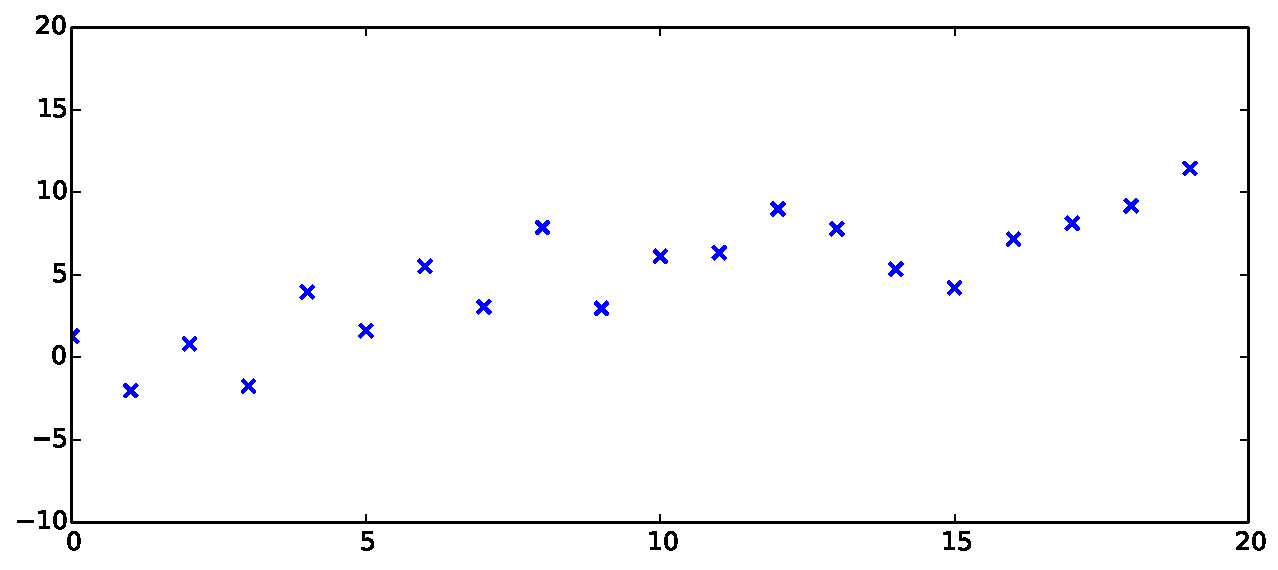
\includegraphics[height=4cm]{figures/2_example}
\end{center}
\end{example}
\end{frame}

%%%%%%%%%%%%%%%%%%%%%%%%%%%%%%%%%%%%%%%%%%%%%%%%%%%%%%
\begin{frame}{}
A time series can show various patterns or features:
\begin{itemize}
	\item centred 
	\item trend
	\item seasonal
	\item cyclical
	\item stationary
	\item noise
	\item missing data
\end{itemize}
\vspace{2mm}
We will now illustrate these features on various examples.
\end{frame}

%%%%%%%%%%%%%%%%%%%%%%%%%%%%%%%%%%%%%%%%%%%%%%%%%%%%%%
\begin{frame}{}
\structure{Centred :} Is the mean value 0 ?\\
\vspace{5mm}
\begin{columns}[c]
\column{5cm}
\begin{center}
Centred
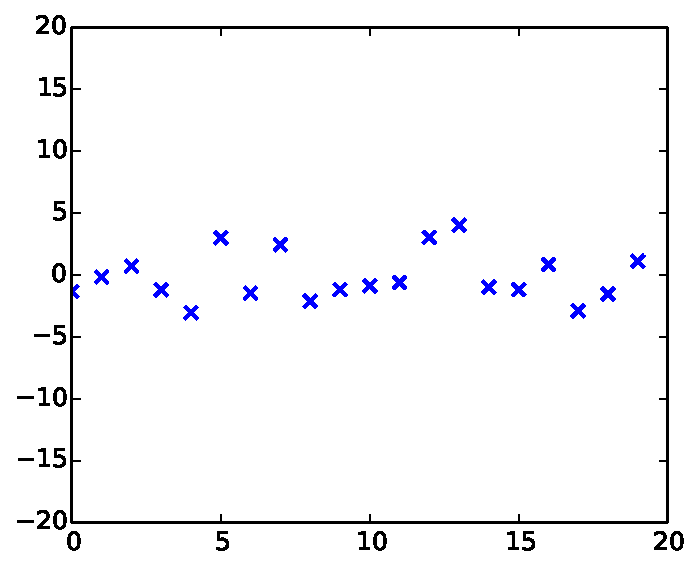
\includegraphics[height=4cm]{figures/2_centred}
\end{center}
\column{5cm}
\begin{center}
Not centred
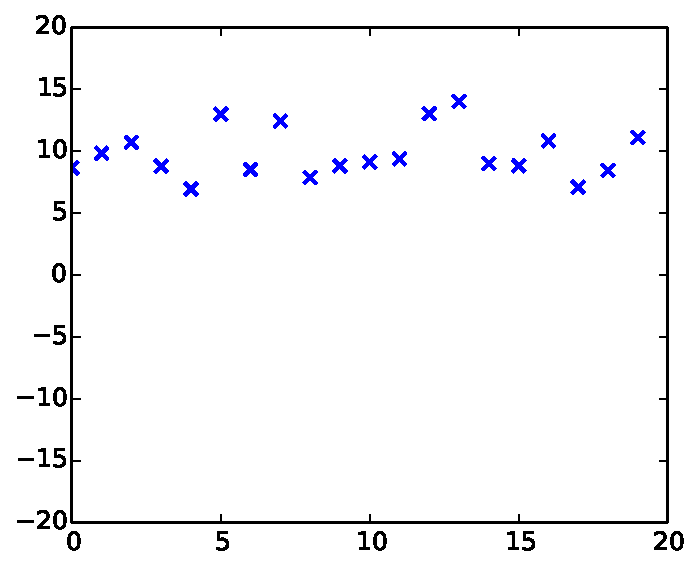
\includegraphics[height=4cm]{figures/2_centredno}
\end{center}
\end{columns}
\end{frame}


%%%%%%%%%%%%%%%%%%%%%%%%%%%%%%%%%%%%%%%%%%%%%%%%%%%%%%
\begin{frame}{}
\structure{Trend :} It is often the most obvious pattern\\
\vspace{5mm}
\begin{columns}[c]
\column{5cm}
\begin{center}
Without trend
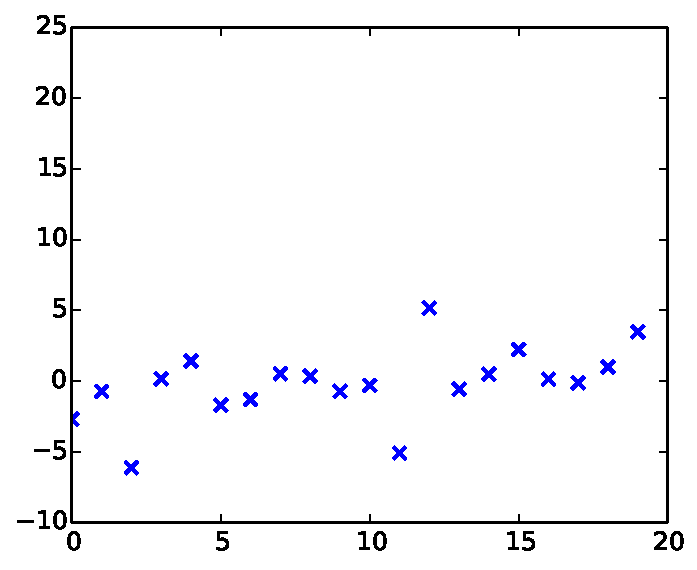
\includegraphics[height=4cm]{figures/2_trendno}
\end{center}
\column{5cm}
\begin{center}
With trend
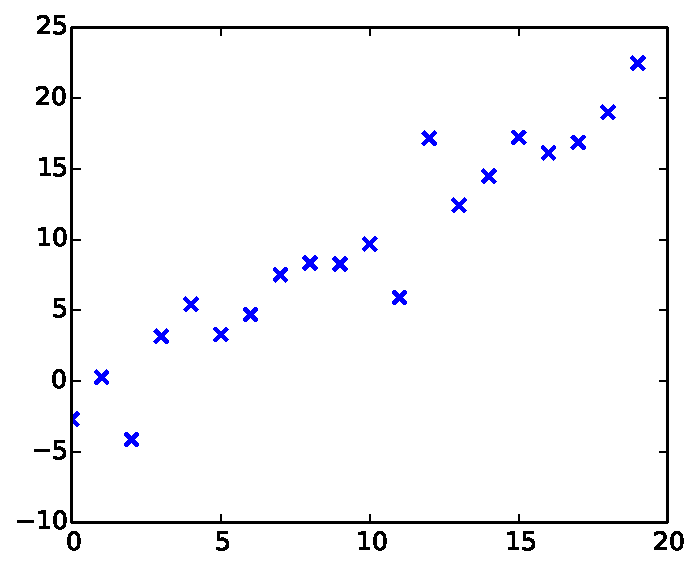
\includegraphics[height=4cm]{figures/2_trend}
\end{center}
\end{columns}
\vspace{5mm}
A trend is not necessarily linear !
\end{frame}

%%%%%%%%%%%%%%%%%%%%%%%%%%%%%%%%%%%%%%%%%%%%%%%%%%%%%%
\begin{frame}{}
\structure{Seasonal :} It is also a pattern that is easy to identify\\
\vspace{5mm}
\begin{columns}[c]
\column{5cm}
\begin{center}
Without seasonality
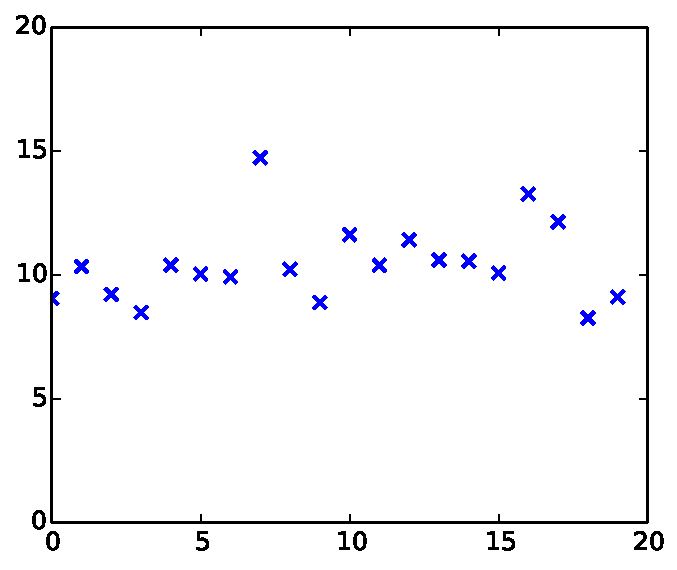
\includegraphics[height=4cm]{figures/2_seasonalno}
\end{center}
\column{5cm}
\begin{center}
With seasonality
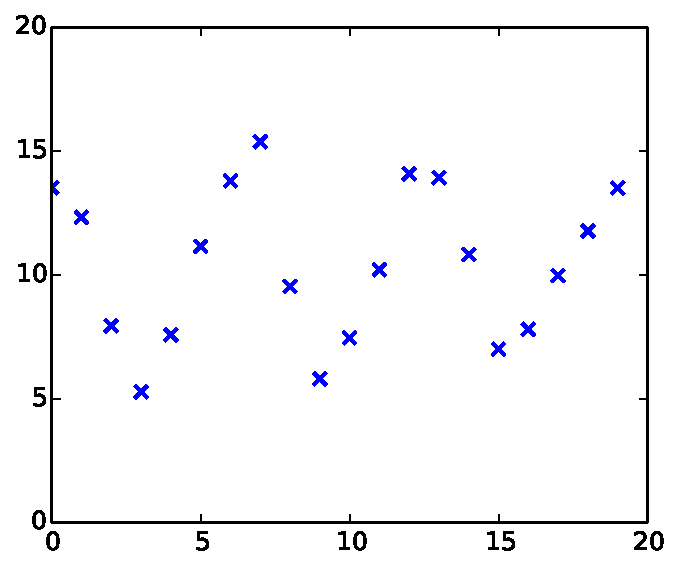
\includegraphics[height=4cm]{figures/2_seasonal}
\end{center}
\end{columns}
\vspace{5mm}
\end{frame}

%%%%%%%%%%%%%%%%%%%%%%%%%%%%%%%%%%%%%%%%%%%%%%%%%%%%%%
\begin{frame}{}
\structure{Cyclical :} Similar to seasonality but not periodic\\
\vspace{5mm}
\begin{columns}[c]
\column{5cm}
\begin{center}
Without cycles
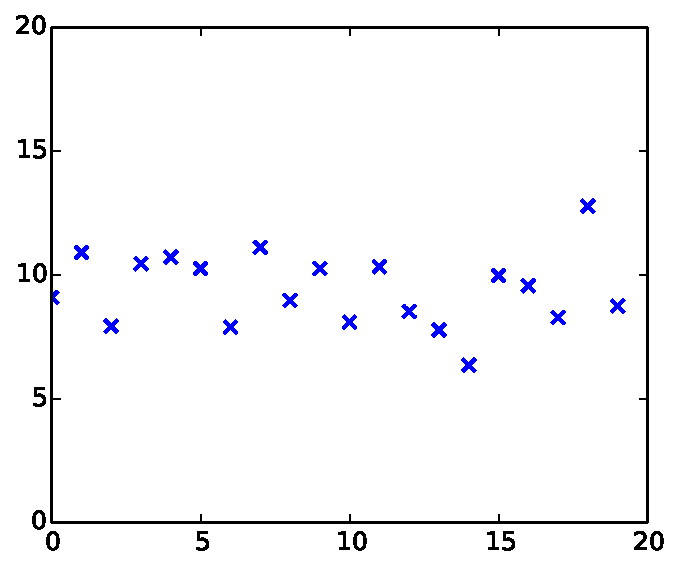
\includegraphics[height=4cm]{figures/2_cyclicalno}
\end{center}
\column{5cm}
\begin{center}
With cycles
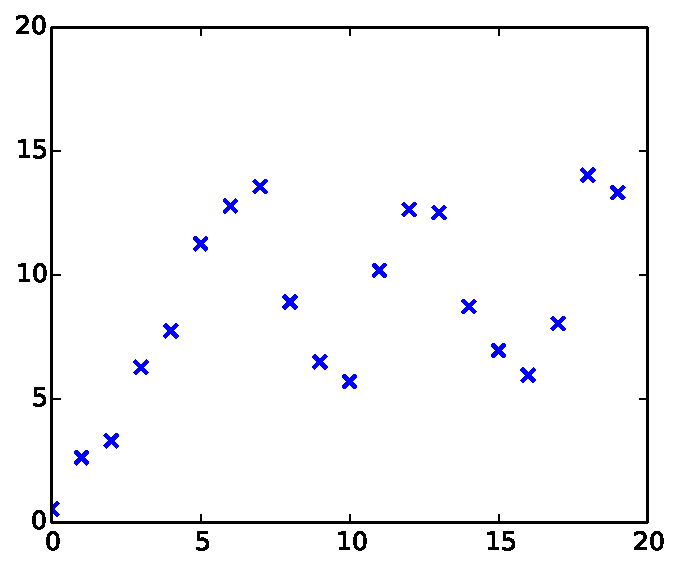
\includegraphics[height=4cm]{figures/2_cyclical}
\end{center}
\end{columns}
\vspace{5mm}
This can make the forecast difficult.
\end{frame}

%%%%%%%%%%%%%%%%%%%%%%%%%%%%%%%%%%%%%%%%%%%%%%%%%%%%%%
\begin{frame}{}
\structure{Stationary :} A time series is stationary when the distribution of $y(t)$ does not change over time.\\
\vspace{5mm}
\begin{columns}[c]
\column{5cm}
\begin{center}
Not stationnary
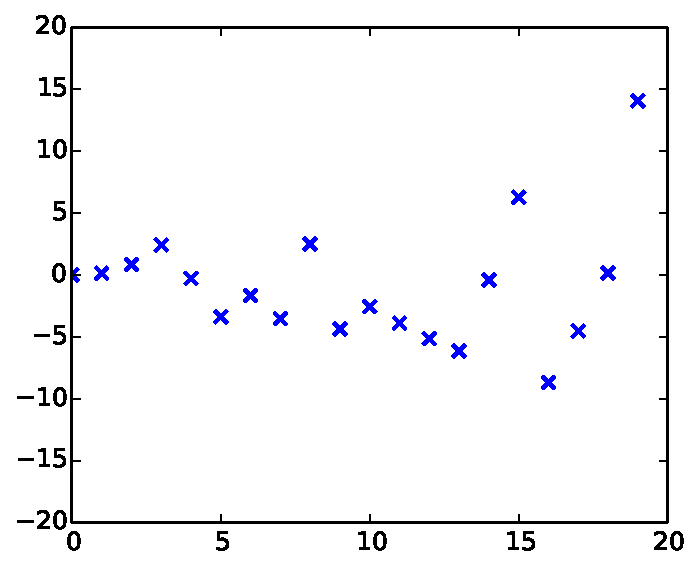
\includegraphics[height=4cm]{figures/2_stationnaryno}
\end{center}
\column{5cm}
\begin{center}
Stationnary
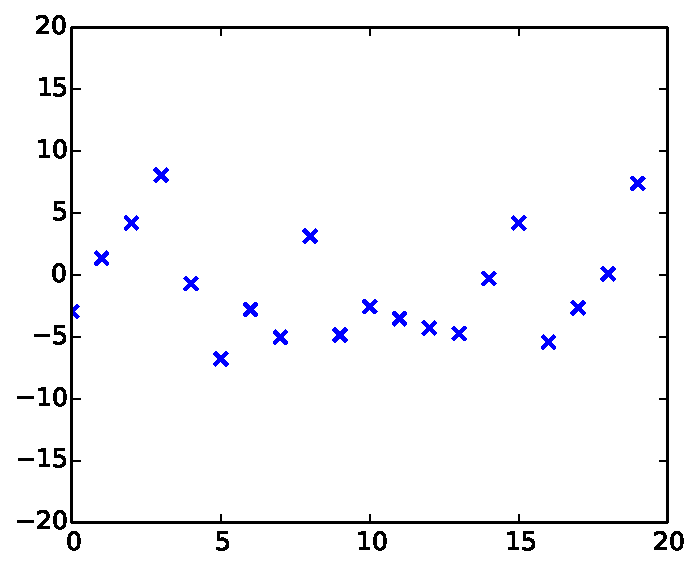
\includegraphics[height=4cm]{figures/2_stationnary}
\end{center}
\end{columns}
\vspace{5mm}
This is a key concept in time series analysis.
\end{frame}

%%%%%%%%%%%%%%%%%%%%%%%%%%%%%%%%%%%%%%%%%%%%%%%%%%%%%%
\begin{frame}{}
\structure{Noise :} Noise is the component of the signal that cannot be explained.\\
\vspace{5mm}
\begin{columns}[c]
\column{5cm}
\begin{center}
Not noisy
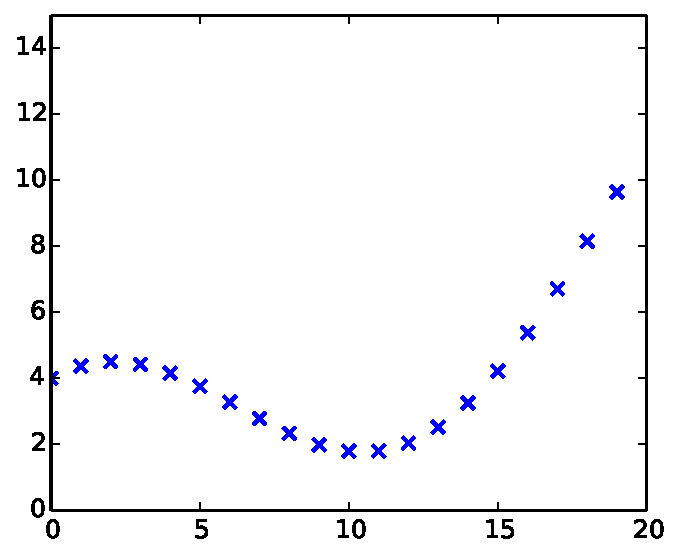
\includegraphics[height=4cm]{figures/2_noisyno}
\end{center}
\column{5cm}
\begin{center}
Noisy
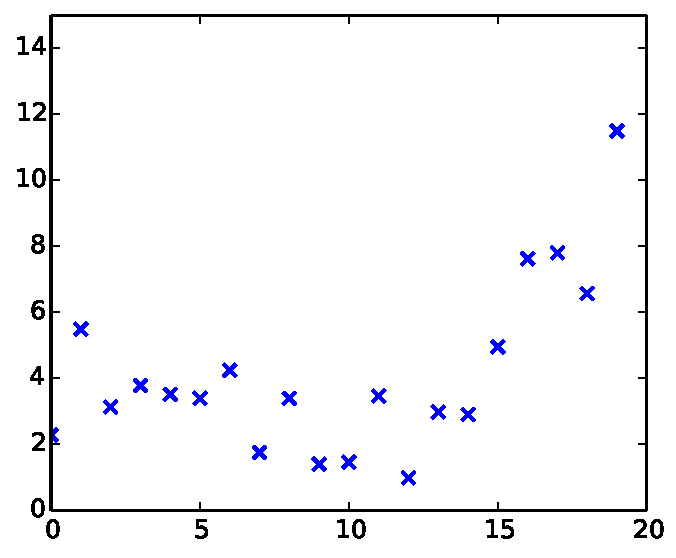
\includegraphics[height=4cm]{figures/2_noisy}
\end{center}
\end{columns}
\vspace{5mm}
It is often difficult to tell if some variations are due to noise.
\end{frame}

%%%%%%%%%%%%%%%%%%%%%%%%%%%%%%%%%%%%%%%%%%%%%%%%%%%%%%
\begin{frame}{}
\structure{Missing data :} In practice, full data is not always available.\\
\vspace{5mm}
\begin{center}
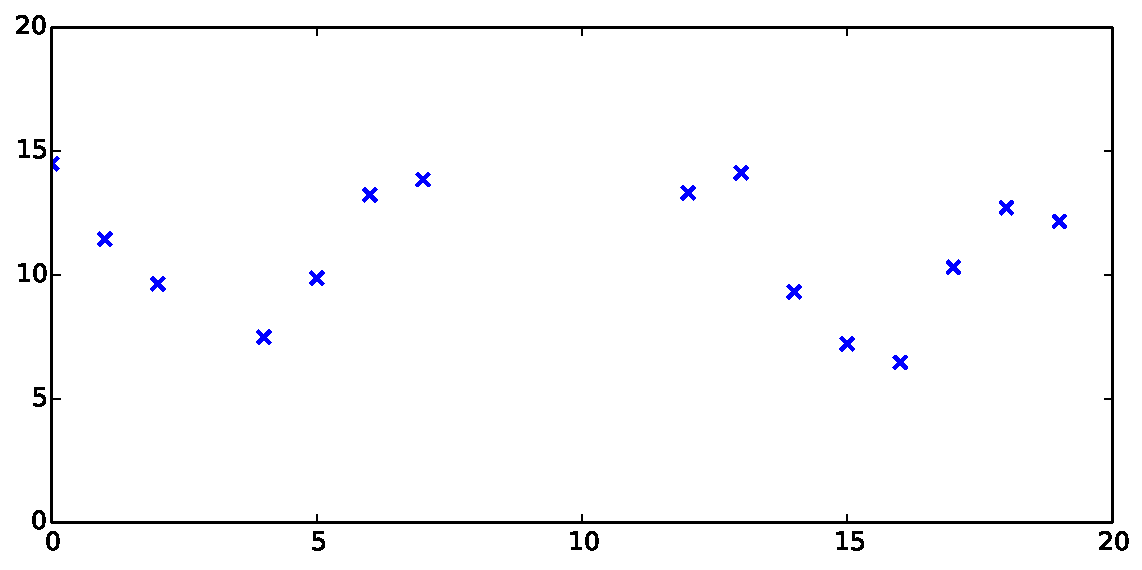
\includegraphics[height=4cm]{figures/2_missing}
\end{center}
\vspace{5mm}
Some methods can cope very well with missing data, others cannot.
\end{frame}

%%%%%%%%%%%%%%%%%%%%%%%%%%%%%%%%%%%%%%%%%%%%%%%%%%%%%%
\begin{frame}{}
\structure{Outliers :} Some of the data may not be reliable.\\
\vspace{5mm}
\begin{center}
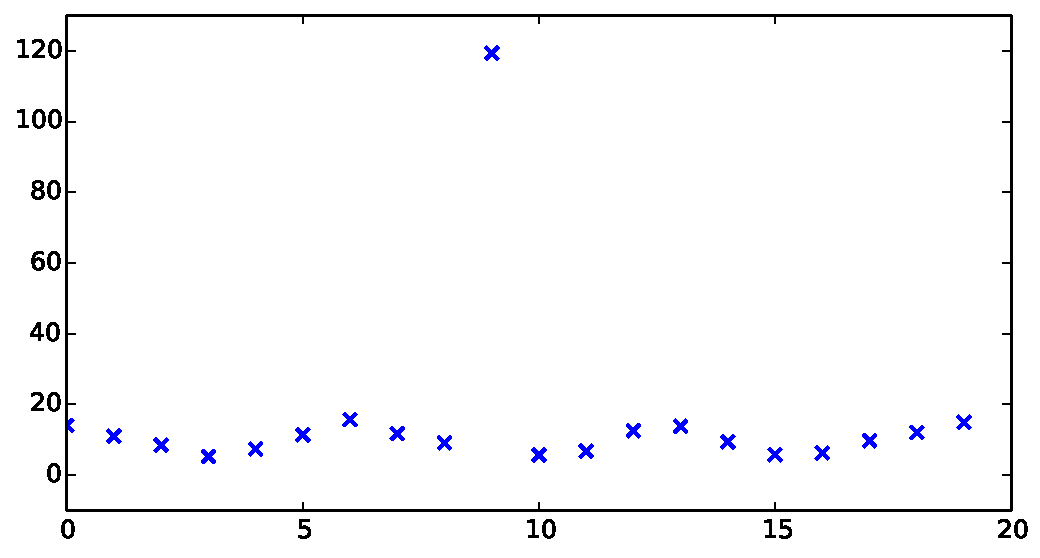
\includegraphics[height=4cm]{figures/2_outliers}
\end{center}
\vspace{5mm}
Outliers should be removed in a preprocessing step.
\end{frame}

%%%%%%%%%%%%%%%%%%%%%%%%%%%%%%%%%%%%%%%%%%%%%%%%%%%%%%
\begin{frame}{}
Most time series show a combinations of the above features:
\begin{center}
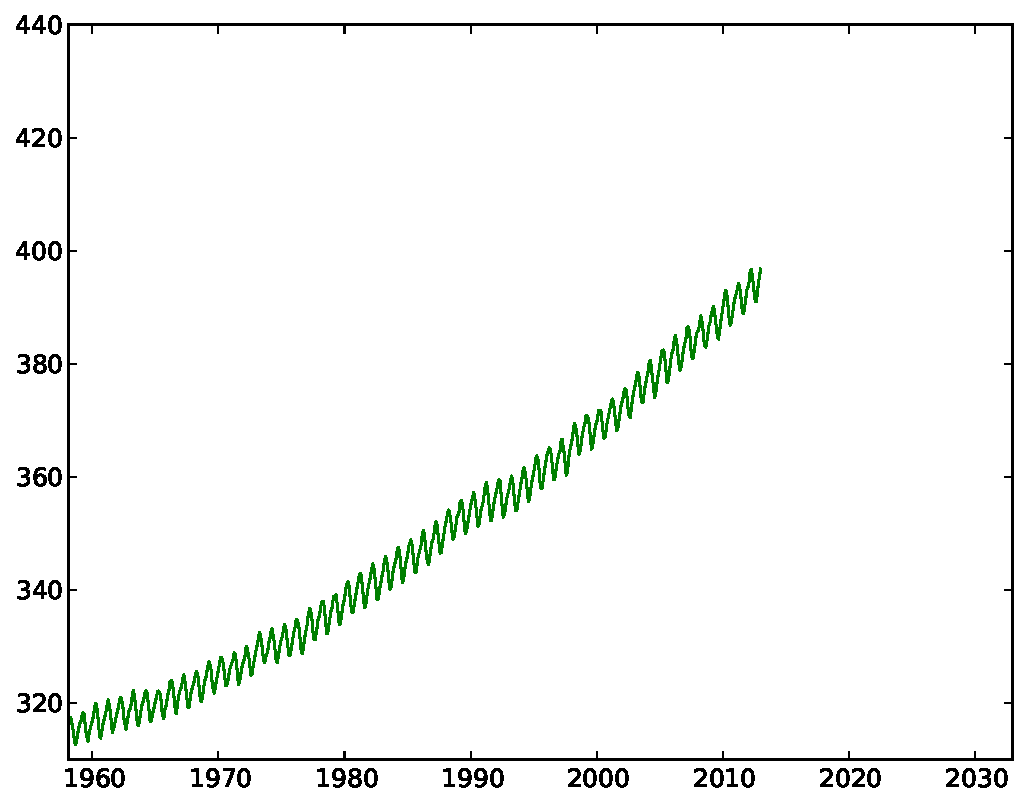
\includegraphics[height=6cm]{figures/CO2-data}\\
$CO_2$ Concentration in the atmosphere in ppm at the Mauna Loa observatory (Hawaii).
\end{center}

\end{frame}

%%%%%%%%%%%%%%%%%%%%%%%%%%%%%%%%%%%%%%%%%%%%%%%%%%%%%%
%%%%%%%%%%%%%%%%%%%%%%%%%%%%%%%%%%%%%%%%%%%%%%%%%%%%%%
\section{Forecasting methods}

%%%%%%%%%%%%%%%%%%%%%%%%%%%%%%%%%%%%%%%%%%%%%%%%%%%%%%
\begin{frame}{}
The quantitative forecasting methods can be divided in two sets:
\begin{columns}[t]
\column{5cm}
\begin{center}
	\textbf{time series models}\\
	\begin{itemize}
		\item Moving average
		\item Exponential smoothing
		\item Autoregressive models
	\end{itemize}
\end{center}
\column{5cm}
\begin{center}
	\textbf{associative models}\\
	\begin{itemize}
		\item Linear regression
	\end{itemize}
\end{center}
\end{columns}
\end{frame}

%%%%%%%%%%%%%%%%%%%%%%%%%%%%%%%%%%%%%%%%%%%%%%%%%%%%%%
\begin{frame}{Moving average}
Moving average is a basic method that can be used for:
\begin{itemize}
	\item noise filtering
	\item missing data prediction
	\item forecasting
\end{itemize}
\vspace{5mm}
The prediction $\hat{y}_t$ at point $t$ is given by the average over the neighbours of $t$:
$$\hat{y}_t = \frac{1}{|V|} \sum_{v \in V} y_v $$
The main question here is how to define a neighbourhood. 
\end{frame}

%%%%%%%%%%%%%%%%%%%%%%%%%%%%%%%%%%%%%%%%%%%%%%%%%%%%%%
\begin{frame}{}
\begin{example}[Denoising]
We consider the following time series that gives the wind velocity (in km/h) every two hours:\\
\begin{center}
  \begin{tabular}{|c|cccccccccc|}
  \hline
  time & 0 	& 2 	& 4 	 & 6 	& 8 	& 10 	& 12 	& 14 	& 16 	& 18 	\\ \hline
  wind & 10	& 3 	& 6 	 & 0 	& 2 	& 7 	& 14 	& 21 	& 17 	& 28 	\\ \hline
  \end{tabular}
\end{center}
\begin{itemize}
	\item What is the smoothed times series if we consider a window $(t-1,t,t+1)$ at time $t$?
	\item Should the smoothing window be large or narrow?
\end{itemize}
\end{example}
\end{frame}

%%%%%%%%%%%%%%%%%%%%%%%%%%%%%%%%%%%%%%%%%%%%%%%%%%%%%%
\begin{frame}{}
\begin{example}[Missing data]
Same data as before with missing observation in 8:\\
\begin{center}
  \begin{tabular}{|c|cccccccccc|}
  \hline
  time & 0 	& 2 	& 4 	 & 6 	& 8 	& 10 	& 12 	& 14 	& 16 	& 18 	\\ \hline
  wind & 10	& 3 	& 6 	 & 0 	&    	& 7 	& 14 	& 21 	& 17 	& 28 	\\ \hline
  \end{tabular}
\end{center}
\begin{itemize}
	\item What smotting window can be considered to predict the missing data?
\end{itemize}
\end{example}
\end{frame}

%%%%%%%%%%%%%%%%%%%%%%%%%%%%%%%%%%%%%%%%%%%%%%%%%%%%%%
\begin{frame}{}
\begin{example}[prediction]
Same settings:\\
\begin{center}
  \begin{tabular}{|c|cccccccccccc|}
  \hline
  time & 0 	& 2 	& 4 	 & 6 	& 8 	& 10 	& 12 	& 14 	& 16 	& 18 	& 20 	& 22 	\\ \hline
  wind & 10	& 3 	& 6 	 & 0 	& 2 	& 7 	& 14 	& 21 	& 17 	& 28 	&   	&   	\\ \hline
  \end{tabular}
\end{center}
\begin{itemize}
	\item What smoothing window can be considered to predict the wind in 20?
	\item What about 22 ?
\end{itemize}
\end{example}
\end{frame}

%%%%%%%%%%%%%%%%%%%%%%%%%%%%%%%%%%%%%%%%%%%%%%%%%%%%%%
\begin{frame}{Weighted Moving average}
Moving average is not very efficient when there is trend in data (see lab session). \\
\vspace{5mm}
An alternative is weighted moving average:
$$\hat{y}_t = \frac{1}{\sum w} \sum_{v \in V} w_{v-t} y_v $$
The weights $w$ are often such that we give less importance to distant observations.
\end{frame}

%%%%%%%%%%%%%%%%%%%%%%%%%%%%%%%%%%%%%%%%%%%%%%%%%%%%%%
\begin{frame}{Exponential smoothing}
One very popular weighted average method is \textbf{exponential smoothing}. In this case, the weights decline exponentially. \\
\vspace{5mm}
The two following definitions are equivalent:
\begin{equation*}
\begin{split}
\hat{y}_t & = \alpha y_{t-1} + \alpha(1-\alpha) y_{t-2} + \dots + \alpha(1-\alpha)^{t-1} y_{0} \\
\hat{y}_t & = \alpha y_{t-1} + (1-\alpha) \hat{y}_{t-1}
\end{split}	
\end{equation*}
The parameter $\alpha$ has to be chosen by the user.
\end{frame}

%%%%%%%%%%%%%%%%%%%%%%%%%%%%%%%%%%%%%%%%%%%%%%%%%%%%%%
\begin{frame}{Exponential smoothing}
Prediction at a two-step horizon is fine when there is no trend in the data :
\begin{center}
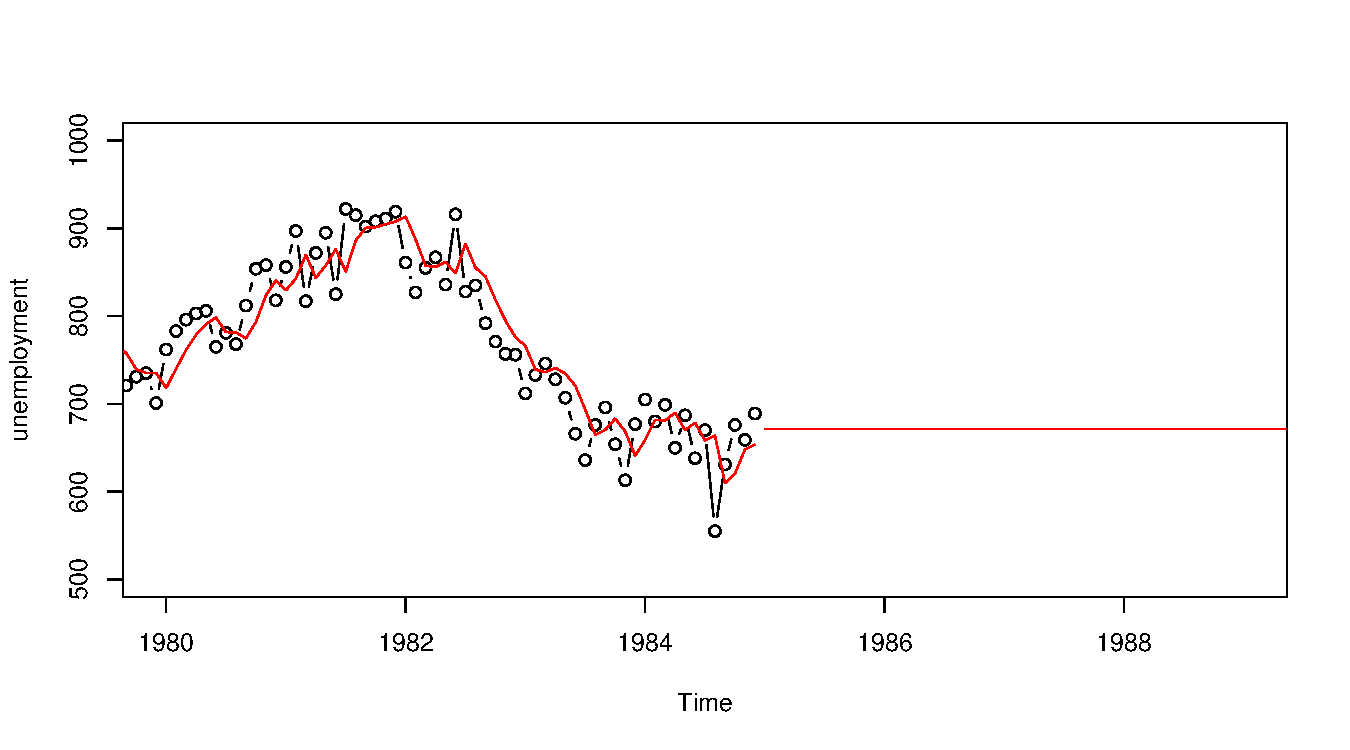
\includegraphics[height=6cm]{figures/R/SESpred}
\end{center}
\end{frame}

%%%%%%%%%%%%%%%%%%%%%%%%%%%%%%%%%%%%%%%%%%%%%%%%%%%%%%
\begin{frame}{Exponential smoothing}
But not very satisfying otherwise:
\begin{center}
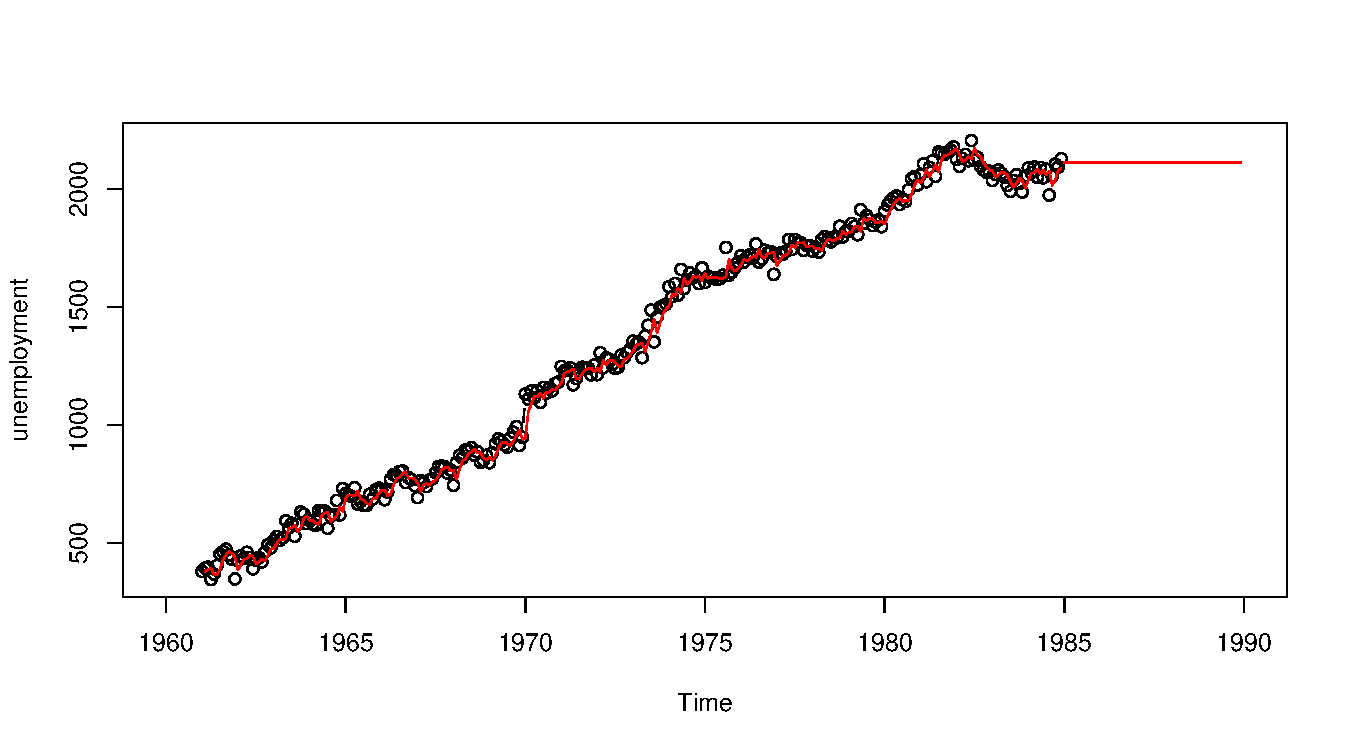
\includegraphics[height=6cm]{figures/R/SESpredtrend}
\end{center}
\end{frame}

%%%%%%%%%%%%%%%%%%%%%%%%%%%%%%%%%%%%%%%%%%%%%%%%%%%%%%
\begin{frame}{Holt-Winters}
Let $\hat{y}(t,h)$ denote the prediction at time $t$ for horizon $h$.\\
\vspace{5mm}
We have just seen that for exponential smoothing 
$$ \hat{y}(t,h) = \hat{a}_t $$
The idea of Holt-Winter algorithm is to have a forecast of the form 
$$ \hat{y}(t,h) = \hat{a}_t + \hat{b}_t h $$
where $\hat{a}$ is called the \emph{level} and $\hat{b}$ the \emph{slope}. These parameters are updated in a similar fashion:
\begin{equation*}
  \begin{split}
    \hat{a}_{t+1} &= \alpha y_{t+1} + (1 - \alpha)(\hat{a}_{t} + \hat{b}_{t}) \\
    \hat{b}_{t+1} &= \beta (\hat{a}_{t+1} - \hat{a}_{t}) + (1 - \beta)\hat{b}_{t}
  \end{split}
\end{equation*}
\end{frame}

%%%%%%%%%%%%%%%%%%%%%%%%%%%%%%%%%%%%%%%%%%%%%%%%%%%%%%
\begin{frame}{Holt-Winters}
Holt-Winters can be initialized with
\begin{itemize}
	\item $\hat{a}_2 = y_2$
	\item $\hat{b}_2 = y_2 - y_1$
\end{itemize}
If we choose $\beta=0$ and $b_2 =0$ we recover exponential smoothing.
\end{frame}

%%%%%%%%%%%%%%%%%%%%%%%%%%%%%%%%%%%%%%%%%%%%%%%%%%%%%%
\begin{frame}{Holt-Winters}
The method is much more adequate in the presence of a trend:
\begin{center}
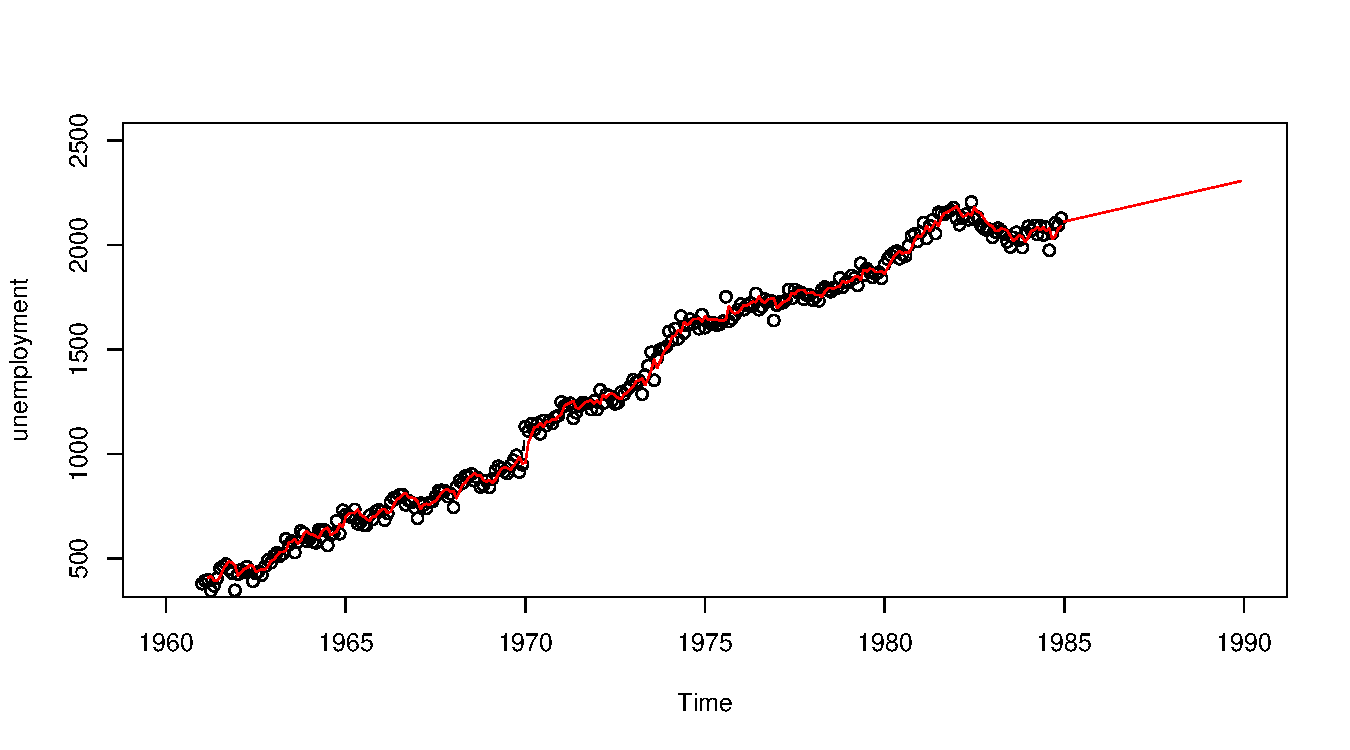
\includegraphics[height=6cm]{figures/R/Holtpredtrend}
\end{center}
\end{frame}


%%%%%%%%%%%%%%%%%%%%%%%%%%%%%%%%%%%%%%%%%%%%%%%%%%%%%%
\begin{frame}{Holt-Winters}
We have just seen that a trend can be added to exponential smoothing. In a similar fashion it is possible to add a seasonality in order to cope with datasets such as
\begin{center}
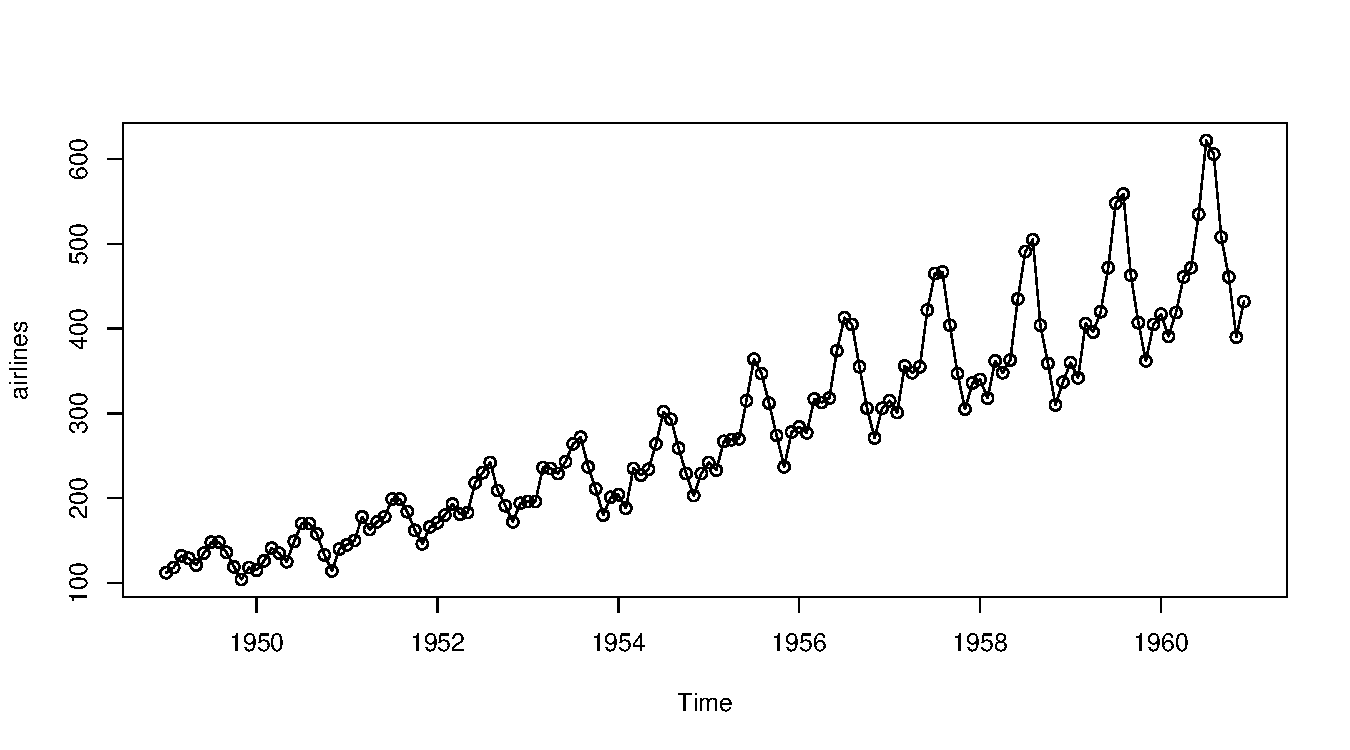
\includegraphics[height=6cm]{figures/R/airlines}
\end{center}
\end{frame}

%%%%%%%%%%%%%%%%%%%%%%%%%%%%%%%%%%%%%%%%%%%%%%%%%%%%%%
\begin{frame}{Holt-Winters}
Holt-Winters seasonal algorithm is based on the smoothing of three components:
\begin{itemize}
	\item The level without seasonality $\hat{a}_n$
	\item The trend slope without seasonality $\hat{b}_n$
	\item The seasonality $\hat{c}_n$
\end{itemize}
\vspace{5mm}
We distinguish two kinds of models
\begin{itemize}
	\item Holt-Winters with additive seasonality
	\item Holt-Winters with multiplicative seasonality
\end{itemize}
The period $s$ is assumed to be known.
\end{frame}

%%%%%%%%%%%%%%%%%%%%%%%%%%%%%%%%%%%%%%%%%%%%%%%%%%%%%%
\begin{frame}{Holt-Winters}
$$ \hat{y}(t,h) = \hat{a}_t + \hat{b}_t h + \hat{c}_{n-ks+h}$$
The updates of $\hat{a}_n$, $\hat{b}_n$ and $\hat{c}_n$ are:
\begin{equation*}
  \begin{split}
    \hat{a}_{t+1} &= \alpha (y_{t+1} -\hat{c}_{t+1-s})  + (1 - \alpha)(\hat{a}_{t} + \hat{b}_{t}) \\
    \hat{b}_{t+1} &= \beta (\hat{a}_{t+1} - \hat{a}_{t}) + (1 - \beta)\hat{b}_{t}\\
    \hat{c}_{t+1} &= \gamma (y_{t+1} -\hat{a}_{t+1}) + (1 - \gamma)\hat{c}_{t+1-d}
  \end{split}
\end{equation*}
\end{frame}


%%%%%%%%%%%%%%%%%%%%%%%%%%%%%%%%%%%%%%%%%%%%%%%%%%%%%%
\begin{frame}{Holt-Winters}
We obtain on the previous example
\begin{center}
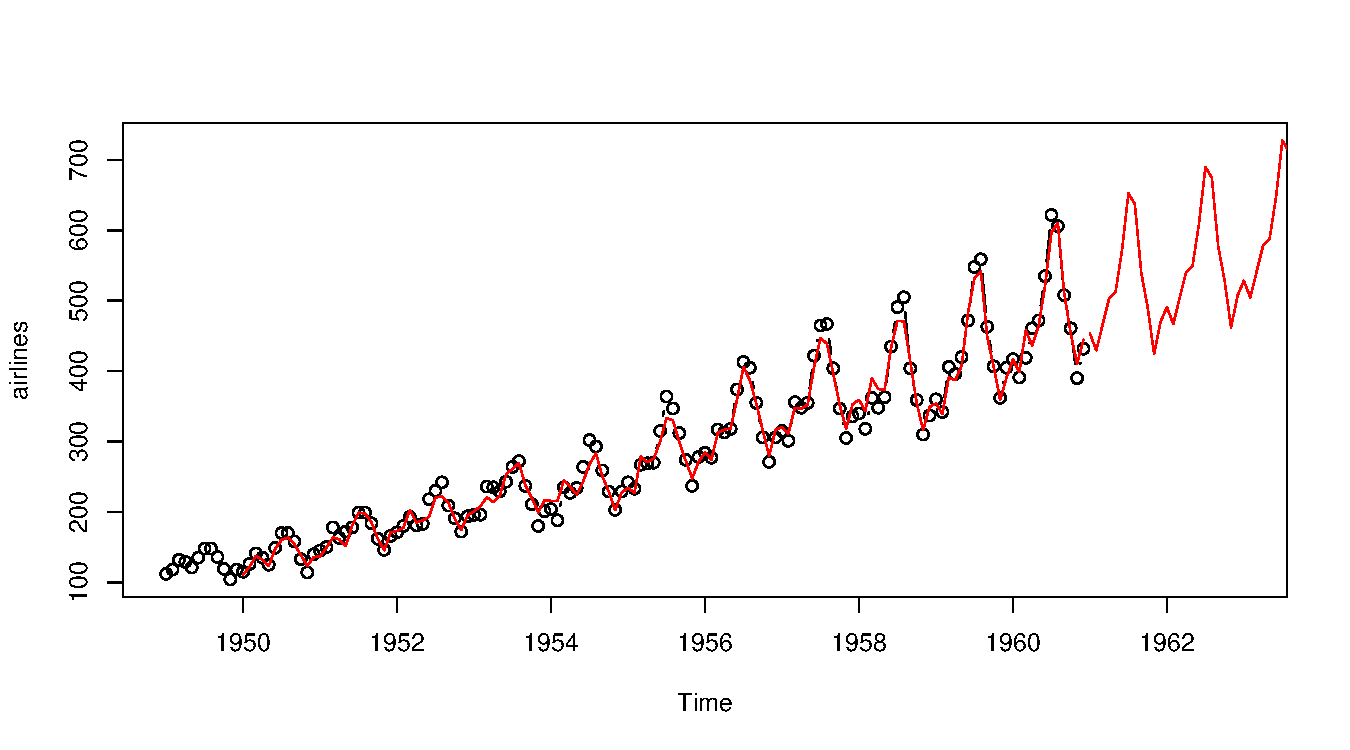
\includegraphics[height=6cm]{figures/R/HoltWintersseasonadd}
\end{center}
\end{frame}

%%%%%%%%%%%%%%%%%%%%%%%%%%%%%%%%%%%%%%%%%%%%%%%%%%%%%%
\begin{frame}{Holt-Winters}
\structure{Holt-Winters with multiplicative seasonality:}\\
$$ \hat{y}(t,h) = (\hat{a}_t + \hat{b}_t h) \hat{c}_{n-ks+h}.$$
The updates of $\hat{a}_n$, $\hat{b}_n$ and $\hat{c}_n$ are:
\begin{equation*}
  \begin{split}
    \hat{a}_{t+1} &= \alpha \frac{y_{t+1}}{\hat{c}_{t+1-s}}  + (1 - \alpha)(\hat{a}_{t} + \hat{b}_{t}) \\
    \hat{b}_{t+1} &= \beta (\hat{a}_{t+1} - \hat{a}_{t}) + (1 - \beta)\hat{b}_{t}\\
    \hat{c}_{t+1} &= \gamma \frac{y_{t+1}}{\hat{a}_{t+1}} + (1 - \gamma)\hat{c}_{t+1-d}
  \end{split}
\end{equation*}
there are $2+s$ initial values that need to be specified.
\end{frame}

%%%%%%%%%%%%%%%%%%%%%%%%%%%%%%%%%%%%%%%%%%%%%%%%%%%%%%
\begin{frame}{Holt-Winters}
We obtain on the previous dataset
\begin{center}
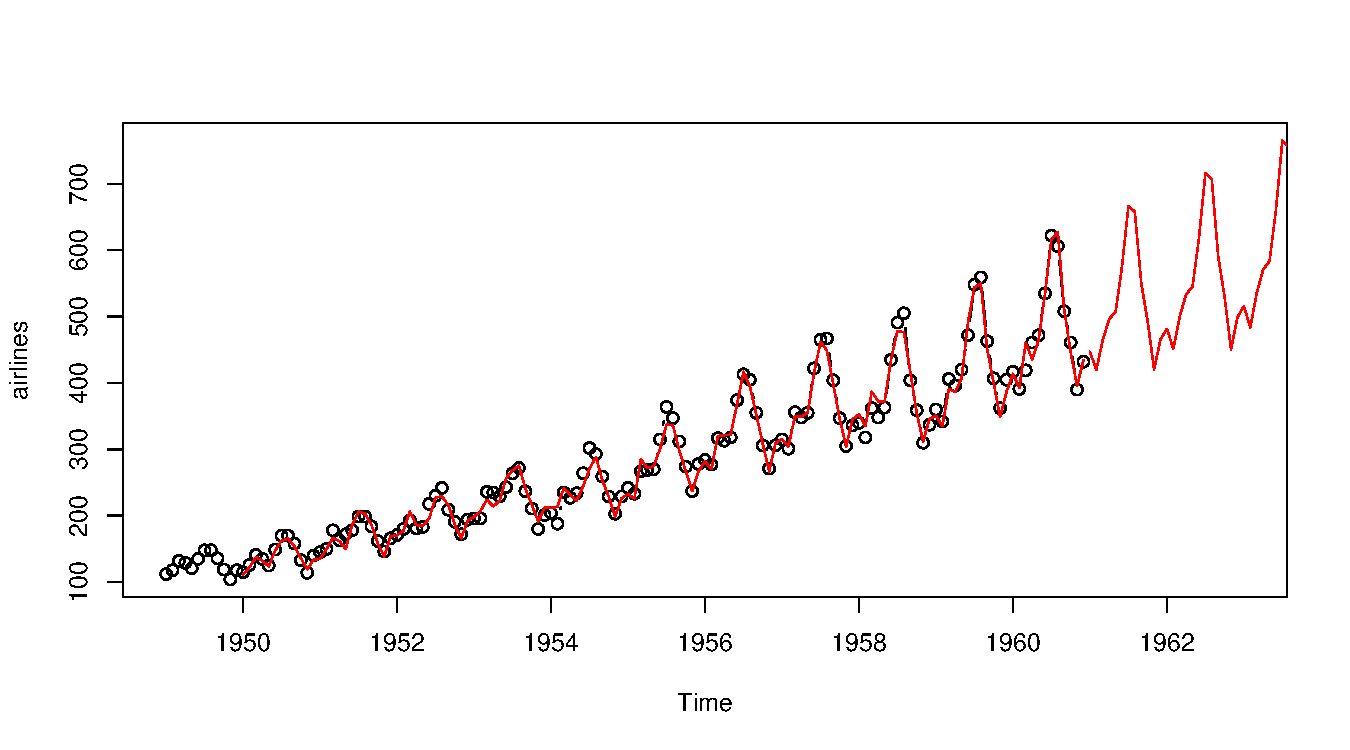
\includegraphics[height=6cm]{figures/R/HoltWintersseasonmult}
\end{center}
\end{frame}

%%%%%%%%%%%%%%%%%%%%%%%%%%%%%%%%%%%%%%%%%%%%%%%%%%%%%%
\begin{frame}{Linear regression}
 Linear regression approximates some observations by a linear combination of basis functions. \\
 \vspace{5mm}
 Let $B(t) = (b_1(t), \dots, b_n(t))$ be the set of basis functions. We look for the function of the form $\hat{y}(t) = B(t) \beta $ that minimises the squared error $\sum (\hat{y}(t_i) - y(t_i))^2$ where the $t_i$ correspond the locations of the observations.\\
 \vspace{5mm}
 If we write $X$ the matrix of general term $X_{i,j} = b_i(t_j)$ and $Y$ the vector of observations, we have $\beta = (X^tX)^{-1}X^t Y$ and thus:
 $$ \hat{y}(t) = B(t) (X^tX)^{-1}X^t Y$$
\end{frame}

%%%%%%%%%%%%%%%%%%%%%%%%%%%%%%%%%%%%%%%%%%%%%%%%%%%%%%
\begin{frame}{Linear regression}
\begin{example}
We consider a basic example :
\begin{center}
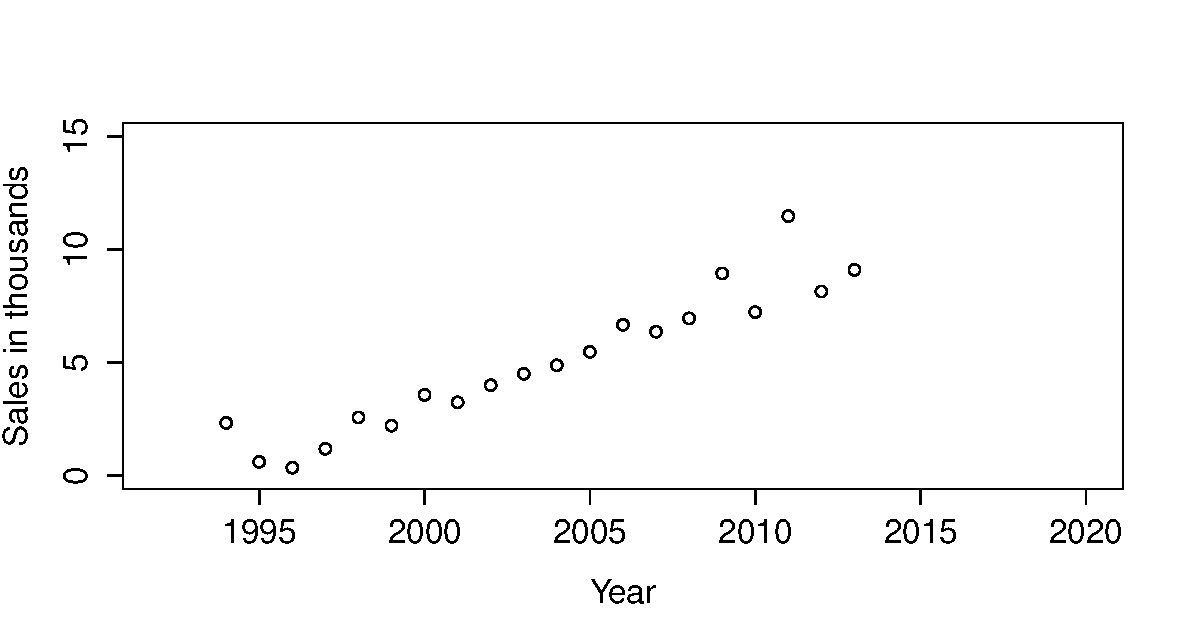
\includegraphics[height=6cm]{figures/3_data}
\end{center}
\end{example}
\end{frame}

%%%%%%%%%%%%%%%%%%%%%%%%%%%%%%%%%%%%%%%%%%%%%%%%%%%%%%
\begin{frame}{Linear regression}
\begin{example}
We use two basis functions :
\begin{center}
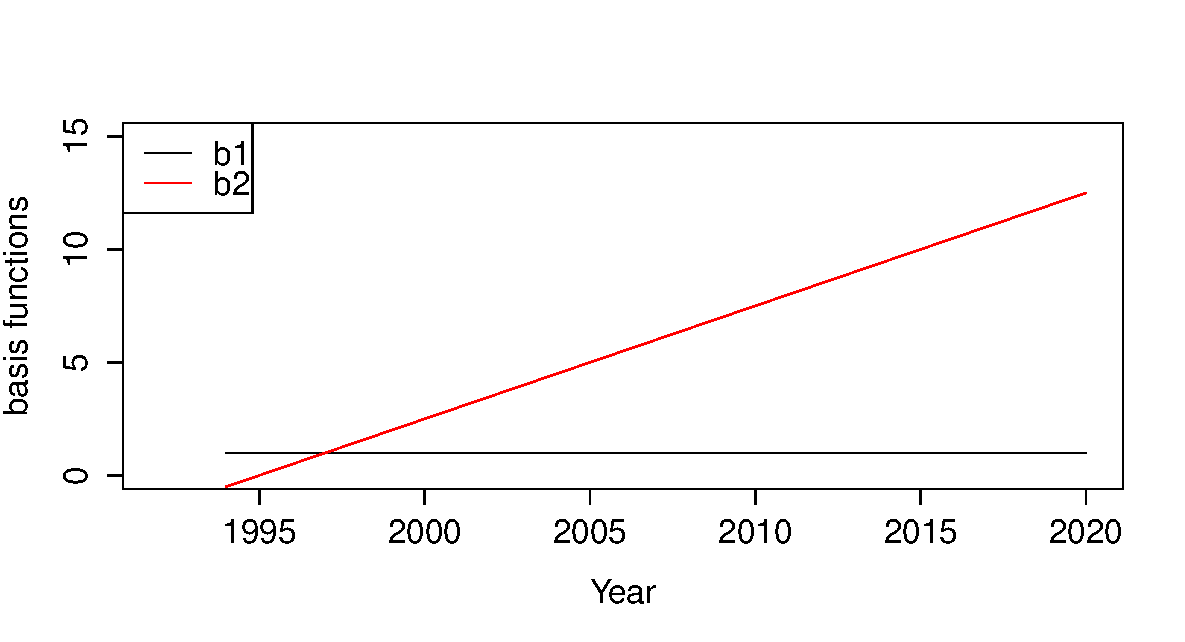
\includegraphics[height=6cm]{figures/3_basis}
\end{center}
\end{example}
\end{frame}

%%%%%%%%%%%%%%%%%%%%%%%%%%%%%%%%%%%%%%%%%%%%%%%%%%%%%%
\begin{frame}{Linear regression}
\structure{Linear regression} \\
\begin{example}
We we obtain the following prediction :
\begin{center}
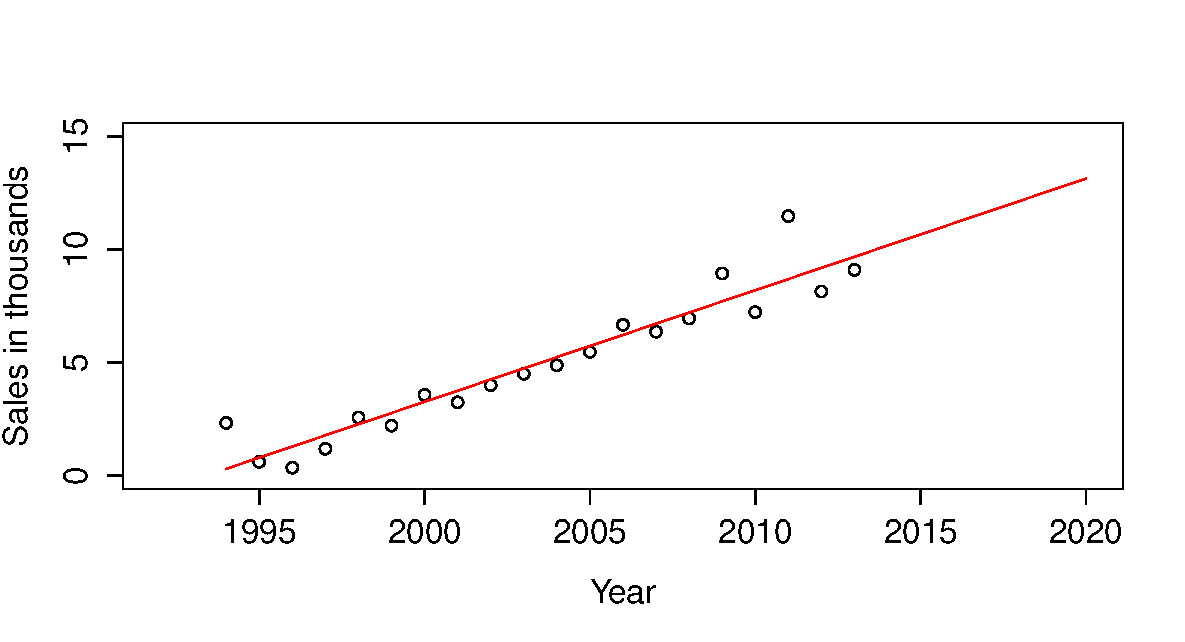
\includegraphics[height=6cm]{figures/3_pred}
\end{center}
\end{example}
\end{frame}

%%%%%%%%%%%%%%%%%%%%%%%%%%%%%%%%%%%%%%%%%%%%%%%%%%%%%%
%%%%%%%%%%%%%%%%%%%%%%%%%%%%%%%%%%%%%%%%%%%%%%%%%%%%%%
\section{Probabilistic models}

%%%%%%%%%%%%%%%%%%%%%%%%%%%%%%%%%%%%%%%%%%%%%%%%%%%%%%
\begin{frame}{}
Up to now, we assumed we had some observations of a variable but we had no \textbf{probabilistic model}.\\
\vspace{5mm}
In this section, we will assume that the \textbf{data we observed is drawn from a random variable}. We will first deal with the case were the distribution of this random variable is known and we will then discuss about its estimation.
\end{frame}

%%%%%%%%%%%%%%%%%%%%%%%%%%%%%%%%%%%%%%%%%%%%%%%%%%%%%%
\begin{frame}{}
We will consider three kinds of probabilistic models
\vspace{2mm}
\begin{itemize}
	\item Autoregressive process (AR) \vspace{2mm}
	\item Moving average process (MA) \vspace{2mm} 
	\item Autoregressive Moving average process (ARMA)
\end{itemize} 
\vspace{5mm}
There are of course many others:
\vspace{2mm}
\begin{itemize}
	\item ARIMA, SARIMA \vspace{2mm}
	\item ARCH, GARCH, TAR
	\item ...
\end{itemize} 
\end{frame}

%%%%%%%%%%%%%%%%%%%%%%%%%%%%%%%%%%%%%%%%%%%%%%%%%%%%%%
\begin{frame}{}
We first need to introduce a couple of notions:\\
\vspace{2mm}
\textbf{random processes} $\{ Z_t \},\ t \in \mathds{N}$ are a generalization of random variables. A sample of a random processes is a series (instead of a value). They are characterised by the joint distribution of the $\{ Z_t \}$.\\
\vspace{2mm}
The mean function $\mu$ and the covariance function $\gamma$ are defined as
\begin{itemize}
 	\item $\mu(t) = E[Z_t]$
 	\item $\gamma(s,t) = \mathrm{cov}(Z_s,Z_t)$
 \end{itemize} 
\vspace{2mm}
A process is (weakly) \textbf{stationary} if 
\begin{itemize}
	\item[(i)] $\mu$ is a constant function
	\item[(ii)] $\gamma(t,t+h) = \gamma(0,h) $
\end{itemize}
In this case, we often write $\gamma$ as a function of one variable $\gamma(s-t)$.

\end{frame}

%%%%%%%%%%%%%%%%%%%%%%%%%%%%%%%%%%%%%%%%%%%%%%%%%%%%%%
\begin{frame}{}
From now we will denote by $Z_t$ the white noise process. It is a process where the $Z_t$ are centred and iid.\\
\vspace{5mm}
\begin{center}
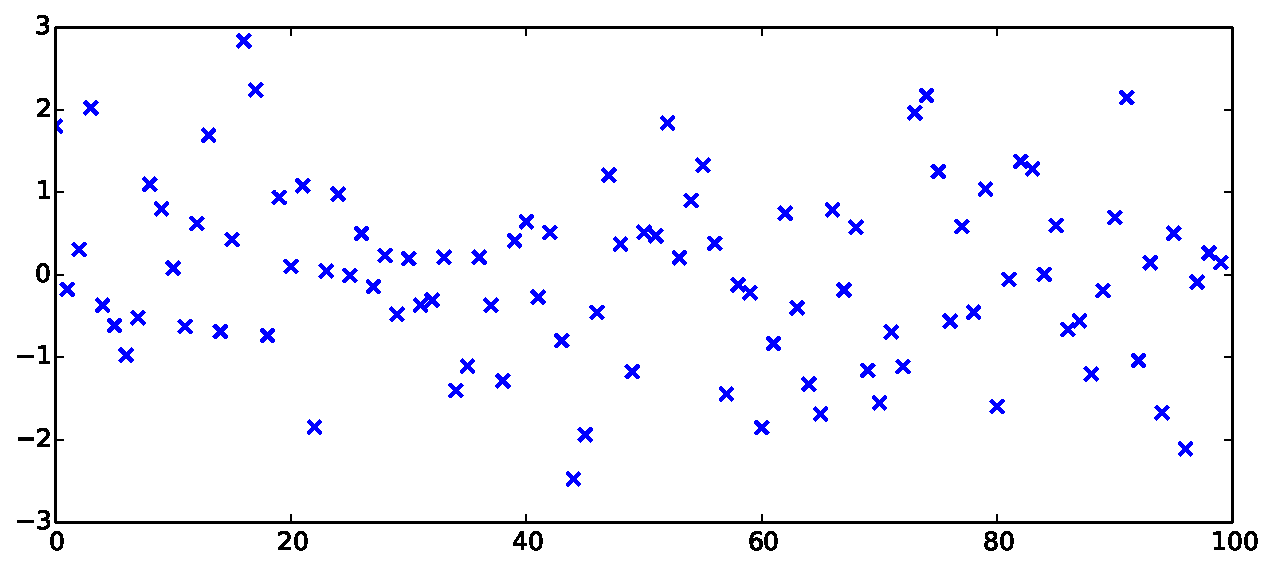
\includegraphics[height=5cm]{figures/1_whitenoise}
\end{center}
\end{frame}

%%%%%%%%%%%%%%%%%%%%%%%%%%%%%%%%%%%%%%%%%%%%%%%%%%%%%%
\begin{frame}{}
\begin{definition}
We call \textbf{moving average process of order $\mathbf{q}$} (MA(q)) any process that can be written as :
\begin{equation*}
X_t  = \alpha_0 Z_{t} + \alpha_1 Z_{t-1} + \dots + \alpha_q Z_{t-q}
%= \sum_{i=0}^{q} \alpha_i Z_{t-i}
\end{equation*}
\end{definition}
They correspond to a moving average filter applied to white noise.
\begin{center}
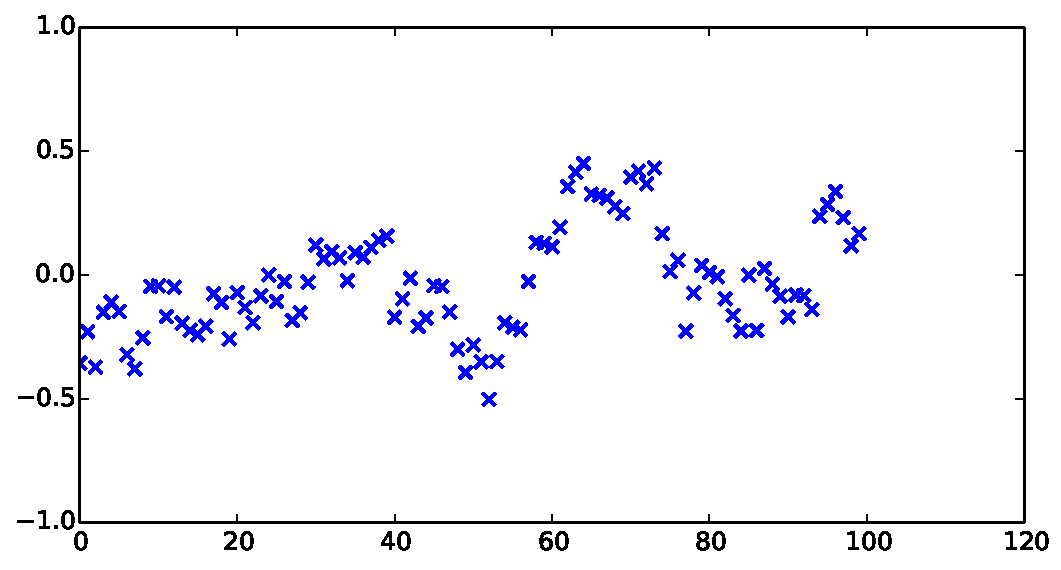
\includegraphics[height=4.5cm]{figures/1_ma}
\end{center}
For this figure we have $w=(1,1,1,1,1,1,1,1,1,1)$.
\end{frame}

%%%%%%%%%%%%%%%%%%%%%%%%%%%%%%%%%%%%%%%%%%%%%%%%%%%%%%
\begin{frame}{}
\begin{exampleblock}{Exercise}
Given a \textbf{moving average process} 
\begin{equation*}
X_t  = \alpha_0 Z_{t} + \alpha_1 Z_{t-1} + \dots + \alpha_q Z_{t-q}
%= \sum_{i=0}^{q} \alpha_i Z_{t-i}
\end{equation*}
\begin{itemize}
	\item Is $X$ a stationary process?
	\item What is the covariance? $\gamma(h) = \mathrm{cov}(X_t,X_{t+h})$?
\end{itemize}
\end{exampleblock}
\pause
The answers are
\begin{itemize}
	\item Yes.
	\item $\gamma(h) = \mathrm{cov}(X_t,X_{t+h}) = \sigma^2 \sum_{i=0}^{q-h} \alpha_i \alpha_{i+h}$
\end{itemize}
\vspace{2mm}
In particular, the covariance is null for $h>q$.
\end{frame}

%%%%%%%%%%%%%%%%%%%%%%%%%%%%%%%%%%%%%%%%%%%%%%%%%%%%%%
\begin{frame}{}
\begin{definition}
We call \textbf{autoregressive process of order $\mathbf{p}$} any process that can be written as :
\begin{equation*}
 X_t - \alpha_1 X_{t-1} - \dots - \alpha_p X_{t-p} = \alpha_0 Z_{t} 
\end{equation*}
\end{definition}
This process can be seen as the solution of a discretized differential operator.
\end{frame}

%%%%%%%%%%%%%%%%%%%%%%%%%%%%%%%%%%%%%%%%%%%%%%%%%%%%%%
\begin{frame}{}
\begin{exampleblock}{Example 1/3: AR(1)}
We consider
\begin{equation*}
 X_t - 0.8 X_{t-1} = Z_{t} 
\end{equation*}
\end{exampleblock}
\begin{center}
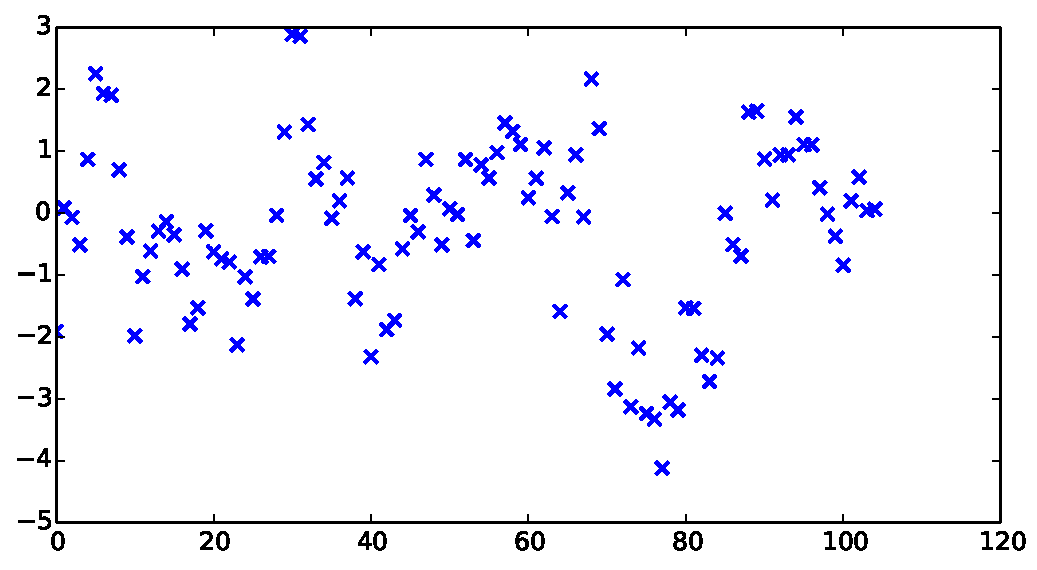
\includegraphics[height=5cm]{figures/1_ar1a}
\end{center}
\end{frame}

%%%%%%%%%%%%%%%%%%%%%%%%%%%%%%%%%%%%%%%%%%%%%%%%%%%%%%
\begin{frame}{}
\begin{exampleblock}{Example 2/3: AR(1)}
Special case : A random walk
\begin{equation*}
 X_t - X_{t-1} = Z_{t} 
\end{equation*}
\end{exampleblock}
\begin{center}
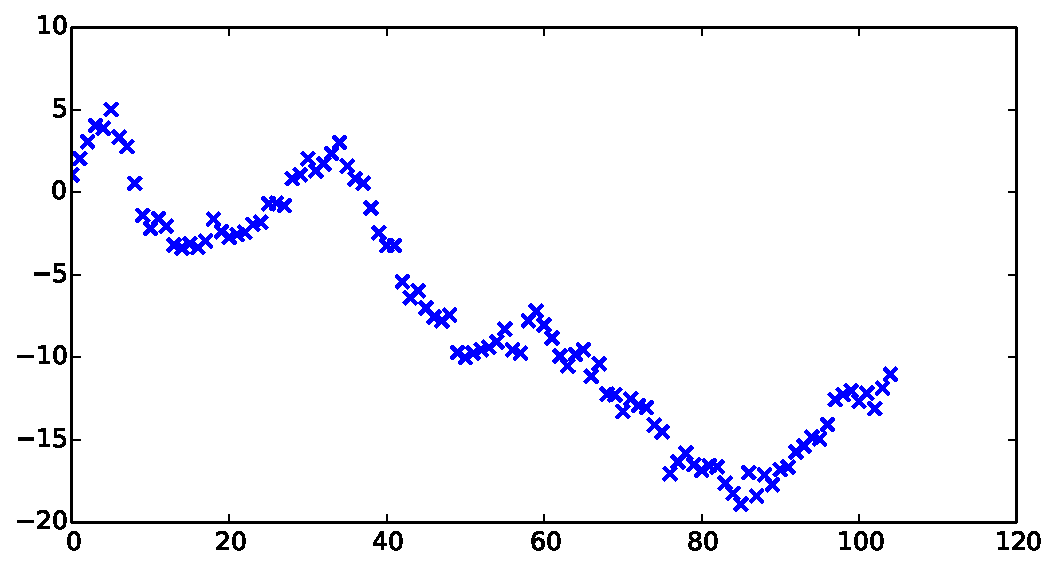
\includegraphics[height=5cm]{figures/1_ar1}
\end{center}
\end{frame}


%%%%%%%%%%%%%%%%%%%%%%%%%%%%%%%%%%%%%%%%%%%%%%%%%%%%%%
\begin{frame}{}
\begin{exampleblock}{Example 3/3: AR(2)}
We consider
\begin{equation*}
 X_t - 2 X_{t-1} + X_{t-2} = Z_{t} 
\end{equation*}
\end{exampleblock}
\begin{center}
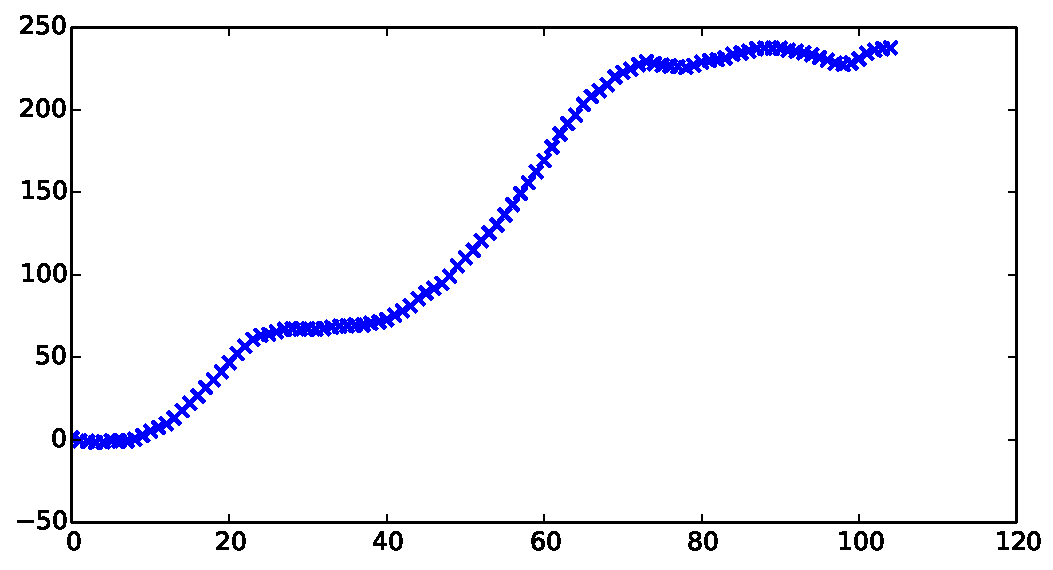
\includegraphics[height=5cm]{figures/1_ar2}
\end{center}
\end{frame}

%%%%%%%%%%%%%%%%%%%%%%%%%%%%%%%%%%%%%%%%%%%%%%%%%%%%%%
\begin{frame}{}
Let $X_t$ be an AR(1) process:
\begin{equation*}
 X_t - \alpha X_{t-1} = Z_{t}, 
\end{equation*}
then $X_t$ is stationary if $\alpha \neq 1$.\\
\vspace{5mm}
Furthermore, if $\alpha < 1$, $X_t$ can also be written as a $MA(\infty)$ process:
\begin{equation*}
 X_t = \sum_{j=0}^\infty \alpha^j Z_{t-j}, 
\end{equation*}
\end{frame}

%%%%%%%%%%%%%%%%%%%%%%%%%%%%%%%%%%%%%%%%%%%%%%%%%%%%%%
\begin{frame}{}
The AR and MA processes can be generalized as ARMA processes
\begin{definition}
We call \textbf{autoregressive moving average process of order $\mathbf{p},\mathbf{q}$} any process $X$ that can be written as :
\begin{equation*}
X_t - \alpha_1 X_{t-1} - \dots - \alpha_p X_{t-p}  = \beta_0 Z_{t} + \beta_1 Z_{t-1} + \dots + \beta_q Z_{t-q}
%= \sum_{i=0}^{q} \alpha_i Z_{t-i}
\end{equation*}
\end{definition}
This class of processes is very famous in time series analysis. The forecasting methods we have just seen can directly be applied to ARMA processes.
\end{frame}


%%%%%%%%%%%%%%%%%%%%%%%%%%%%%%%%%%%%%%%%%%%%%%%%%%%%%%
%%%%%%%%%%%%%%%%%%%%%%%%%%%%%%%%%%%%%%%%%%%%%%%%%%%%%%
\section{Forecasting}

%%%%%%%%%%%%%%%%%%%%%%%%%%%%%%%%%%%%%%%%%%%%%%%%%%%%%%
\begin{frame}{}
The optimal 1 step ahead forecast is:
\begin{equation*}
\hat{X}_t = E[X_{t}|X_{t-1},\dots,X_0]
\end{equation*}
In practice, we focus on the best linear predictor.
\begin{exampleblock}{Exercise}
\begin{itemize}
	\item Show that, for an AR process, $\hat{X}_t = \alpha_1 X_{t-1} + \dots + \alpha_p X_{t-p}$
	\item What about the two step ahead forecast?
\end{itemize}
\end{exampleblock}

\end{frame}

%%%%%%%%%%%%%%%%%%%%%%%%%%%%%%%%%%%%%%%%%%%%%%%%%%%%%%
\begin{frame}{}
We obtain for the previous examples:
\vspace{5mm}
\begin{columns}[c]
\column{5cm}
\begin{center}
AR(1)\\
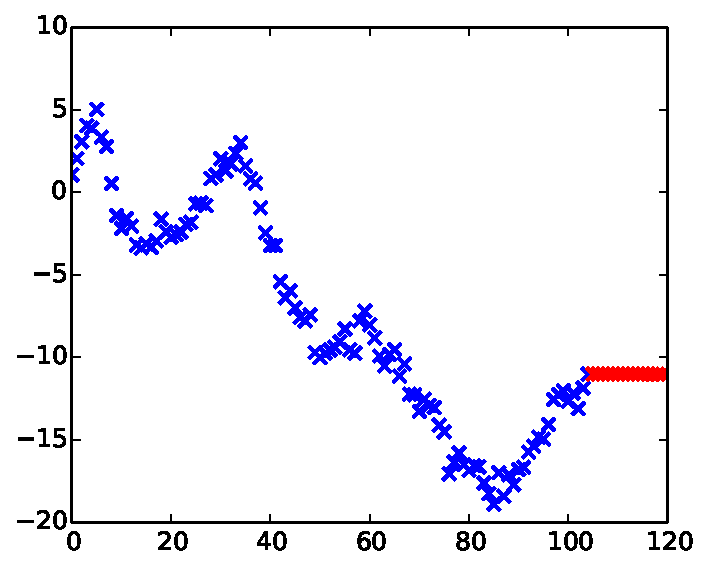
\includegraphics[height=4cm]{figures/1_ar1pred}
\end{center}
\column{5cm}
\begin{center}
AR(2)\\
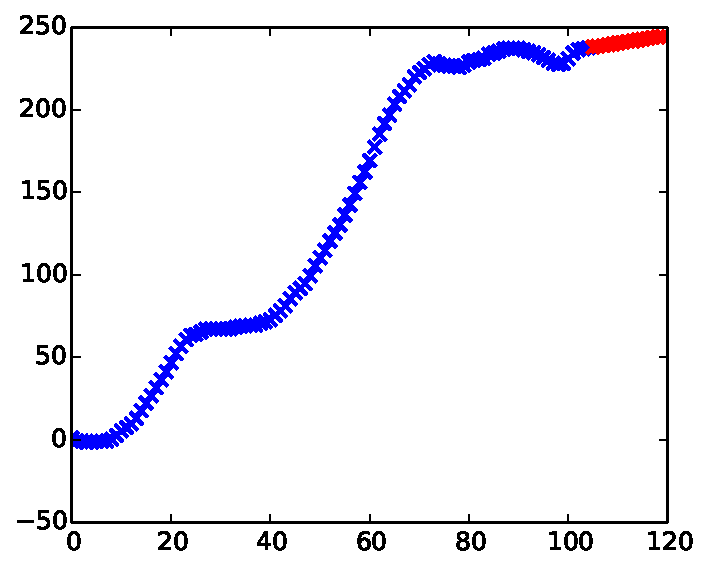
\includegraphics[height=4cm]{figures/1_ar2pred}
\end{center}
\end{columns}
\end{frame}



%%%%%%%%%%%%%%%%%%%%%%%%%%%%%%%%%%%%%%%%%%%%%%%%%%%%%%
\begin{frame}{}
For such process, the optimal forecast is not as straightforward as before. We are looking for the values $a_0, \dots, a_n$ that minimises the error:
$$ E[(X_{n+h} - a_0 - a_1 X_{n} - \dots -  a_n X_{1})^2] = E[(X_{n+h} - \mathbf{a}^t \mathbf{X_{p}})^2]$$
This is quadratic in \textbf{a} so we can differentiate this expression and find where it is null. We finally obtain
\begin{equation*}
	\begin{split}
\mathbf{a} &=  E[\mathbf{X_{p}} \mathbf{X_{p}}^t]^{-1} E[X_{n+h} \mathbf{X_{p}}]\\
&= 
\begin{pmatrix}
	\gamma(0) & \gamma(1) & \dots 	  & \dots & \gamma(n) \\
	\gamma(1) & \gamma(0) & \gamma(1) & \dots & \gamma(n-1) \\
	\vdots    & \ddots    & \ddots    & \ddots & \vdots \\
	\gamma(n) & \gamma(n-1) & \dots & \dots & \gamma(0) 
\end{pmatrix}^{-1}
\begin{pmatrix}
	\gamma(h) \\
	\gamma(h+1) \\
	\vdots    \\
	\gamma(h+n) \\
\end{pmatrix}
	\end{split}
\end{equation*}
\begin{center}
This approach is general and it also stands for AR processes.
\end{center}
\end{frame}

%%%%%%%%%%%%%%%%%%%%%%%%%%%%%%%%%%%%%%%%%%%%%%%%%%%%%%
\begin{frame}{}
If we consider the previous example we obtain:
\begin{center}
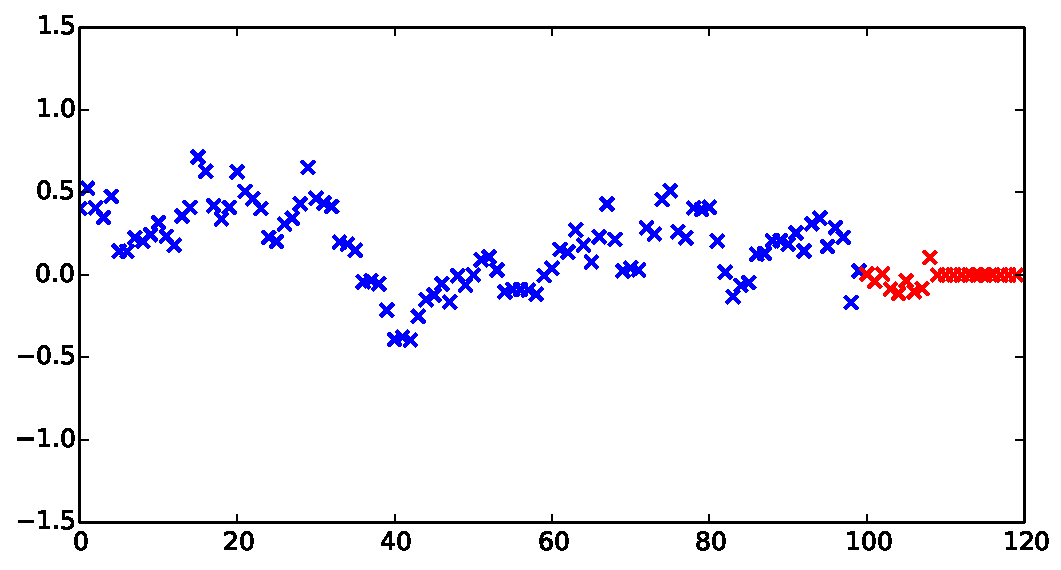
\includegraphics[height=5cm]{figures/1_mapred}
\end{center}
\end{frame}


%%%%%%%%%%%%%%%%%%%%%%%%%%%%%%%%%%%%%%%%%%%%%%%%%%%%%%
\begin{frame}{}
A great asset of probabilistic models is to provide not only a ``mean predictor'' but also a quantification of the uncertainty:
\begin{equation*}
v^2(t,h) = Var[X_{t+h}|X_{t},\dots,X_0]
\end{equation*}
In the Gaussian case, confidence intervals are $mean \pm 1.96 sd$
\begin{center}
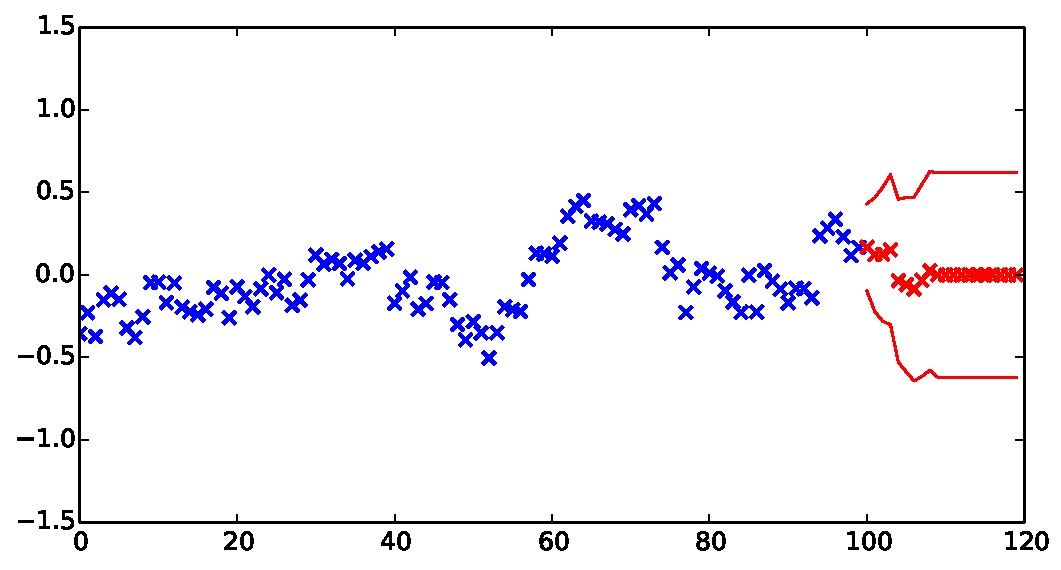
\includegraphics[height=5cm]{figures/1_mapredconf}
\end{center}
\end{frame}

%%%%%%%%%%%%%%%%%%%%%%%%%%%%%%%%%%%%%%%%%%%%%%%%%%%%%%
%%%%%%%%%%%%%%%%%%%%%%%%%%%%%%%%%%%%%%%%%%%%%%%%%%%%%%
\section{Parameters estimation}

%%%%%%%%%%%%%%%%%%%%%%%%%%%%%%%%%%%%%%%%%%%%%%%%%%%%%%
\begin{frame}{}
In the previous section we have seen that the predictions can be made for AR, MA and ARMA models when the autocovariance is known.\\
\vspace{5mm}
In practice, we just observe the data so the model's parameters:
\begin{itemize}
	\item the orders $p$ and $q$ 
	\item the parameters $\alpha_1$, \dots, $\alpha_p$ and $\beta_0$, \dots, $\beta_q$
\end{itemize}
are unknown and they have to be estimated from the data.
\end{frame}

%%%%%%%%%%%%%%%%%%%%%%%%%%%%%%%%%%%%%%%%%%%%%%%%%%%%%%
\begin{frame}{}
We have seen that for $h>q$, the autocorrelation of a MA is null: $\gamma(h)=0$. This can be used to estimate $q$: 
\begin{center}
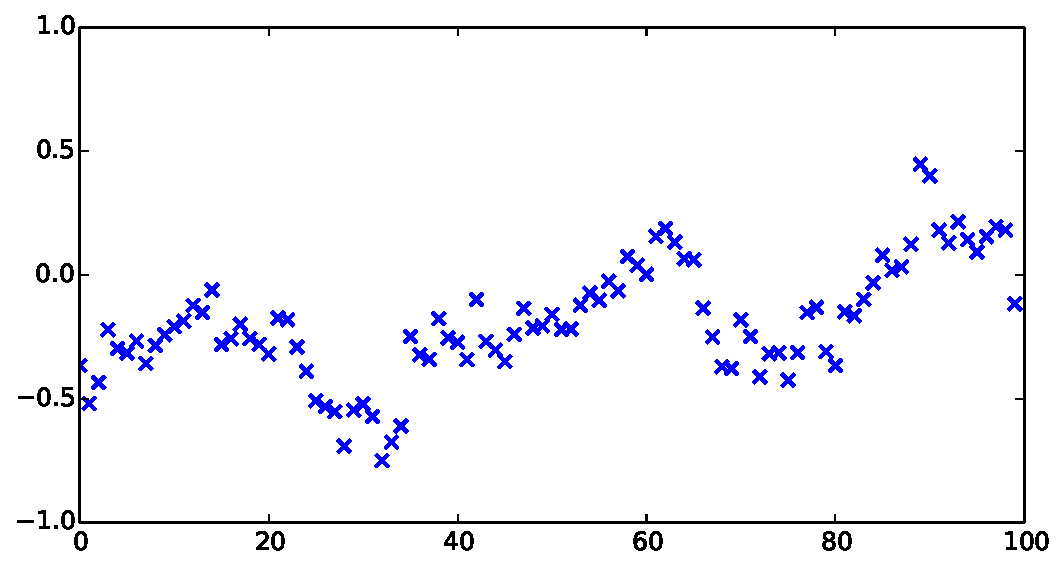
\includegraphics[height=3cm]{figures/1_mab}
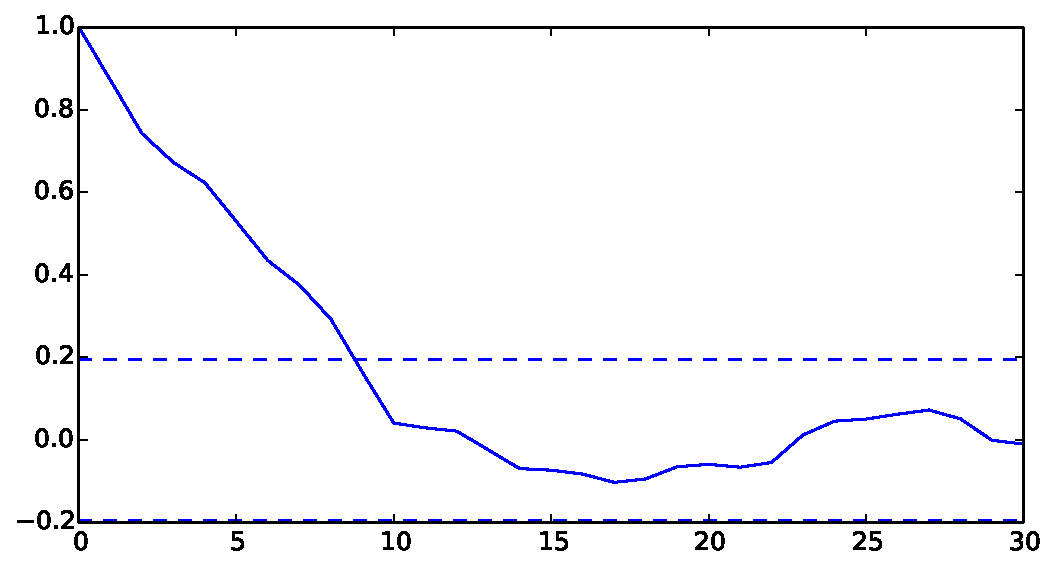
\includegraphics[height=3cm]{figures/1_mabEstQ}
\end{center}
in this example we had $q=10$.
\end{frame}

%%%%%%%%%%%%%%%%%%%%%%%%%%%%%%%%%%%%%%%%%%%%%%%%%%%%%%
\begin{frame}{}
In a similar fashion, for $h>q$, the \emph{partial autocorrelation} of an AR is null $\pi(h)=0$, where
\small
\begin{equation*}
	\pi(h) = corr(X_{t} - E[X_{t}|X_{t+1},...,X_{t+h-1}] \ , \ X_{t+h} - E[X_{t+h}|X_{t+1},...,X_{t+h-1}])
\end{equation*}
\normalsize
This can be used to estimate $p$.
\end{frame}

%%%%%%%%%%%%%%%%%%%%%%%%%%%%%%%%%%%%%%%%%%%%%%%%%%%%%%
\begin{frame}{}
Various methods allow to estimate the model parameters:
\begin{itemize}
	\item Computation of the \emph{sample autocovariance function} and \emph{sample partial autocovariance function}.
	\item least square estimation
	\item maximum likelihood estimation
\end{itemize}
We do not have time do detail these methods which are already implemented in various packages.
\end{frame}


%%%%%%%%%%%%%%%%%%%%%%%%%%%%%%%%%%%%%%%%%%%%%%%%%%%%%%
%%%%%%%%%%%%%%%%%%%%%%%%%%%%%%%%%%%%%%%%%%%%%%%%%%%%%%
\section[Model validation]{Assessing the prediction quality}

%%%%%%%%%%%%%%%%%%%%%%%%%%%%%%%%%%%%%%%%%%%%%%%%%%%%%%
\begin{frame}{}
A good forecast is a forecast that has a small prediction error. This can be measured with the Mean Square Error :
$$ MSE = \frac1n\sum_{i=1}^n (\hat{y}(t_i) - y(t_i))^2$$
In order to measure this quantity, we can compare the \textbf{forecast with reality on past data}. \\
\vspace{5mm}
\begin{columns}[c]
\column{5cm}
Furthermore, if the model provides some uncertainty measure on the forecasts, it is important to validate it as well:
\column{5cm}
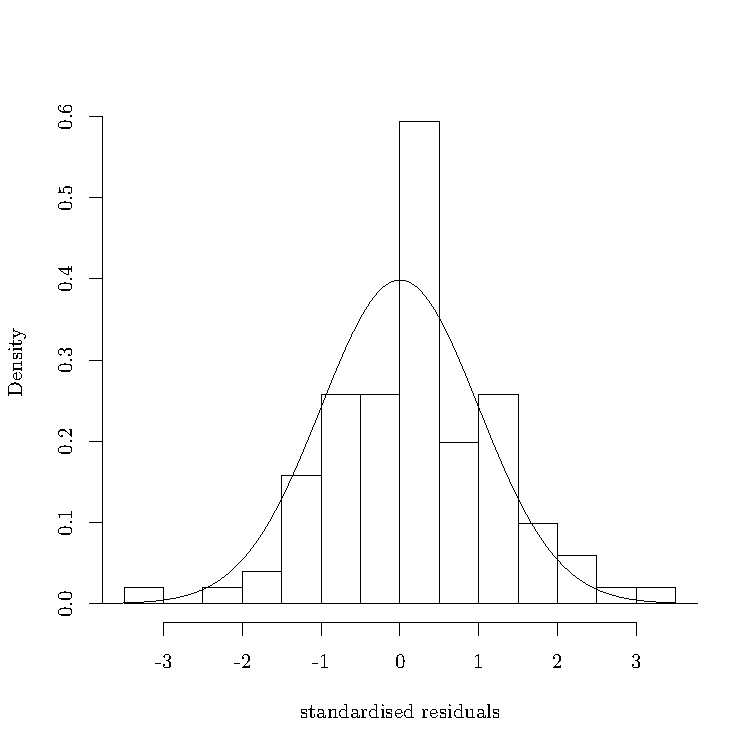
\includegraphics[height=5cm]{figures/VALID_hist.pdf}
\end{columns}
\end{frame}

%%%%%%%%%%%%%%%%%%%%%%%%%%%%%%%%%%%%%%%%%%%%%%%%%%%%%%
%%%%%%%%%%%%%%%%%%%%%%%%%%%%%%%%%%%%%%%%%%%%%%%%%%%%%%
\section{Conclusion}

%%%%%%%%%%%%%%%%%%%%%%%%%%%%%%%%%%%%%%%%%%%%%%%%%%%%%%
\begin{frame}{}
Three important points to remember :\\
\vspace{2mm}
\begin{itemize}
	\item Forecasts \textbf{cannot be perfect} but we want them to be \textbf{as accurate as possible} \vspace{2mm}
	\item Time series analysis is a well suited framework for prediction \vspace{2mm}
	\item \textbf{Validating the model} is of the utmost importance. It can be done on past data.
\end{itemize}
\vspace{8mm}
We will illustrate these notions during next week lab session.
\end{frame}

%%%%%%%%%%%%%%%%%%%%%%%%%%%%%%%%%%%%%%%%%%%%%%%%%%%%%%
\begin{frame}{}
Finally
\vspace{2mm}
\begin{itemize}
	\item The probabilistic framework is of great interest in forecasting
	\begin{itemize}
	 	\item it allows to study the optimality of a forecast
	 	\item it can be used to estimate parameters
	\end{itemize}  \vspace{2mm}
	\item Advanced models such as ARMA or Holt-Winters can capture specific patterns such as trend or seasonality \vspace{2mm}
	\item Methods are already implemented in statistical software
\end{itemize}
\end{frame}



\end{document}
%%%%%%%%%%%%%%%%%%%%%%%%%%%%%%%%%%%%%%%%%%%%%%%%%%%%%%
%%%%%%%%%%%%%%%%%%%%%%%%%%%%%%%%%%%%%%%%%%%%%%%%%%%%%%
%%%%%%%%%%%%%%%%%%%%%%%%%%%%%%%%%%%%%%%%%%%%%%%%%%%%%%

###
%%%%%%%%%%%%%%%%%%%%%%%%%%%%%%%%%%%%%%%%%%%%%%%%%%%%%%
\begin{frame}{}

\end{frame}

###
\begin{block}{}

\end{block}

###
\structure{}

###
\begin{center}
  \begin{tabular}{|c|cc|}

  \end{tabular}
\end{center}

###
\begin{center}
\includegraphics[height=5cm]{figures/}
\end{center}

###
\begin{columns}[c]
\column{5cm}

\column{5cm}

\end{columns}
